% Master report
%
% Dates : 
%   - Submission :          01/09/2012
%
%
%
%\documentclass{llncs}
%
%\usepackage{graphicx}
%\usepackage{url}
%\usepackage{alltt}
%\usepackage{latexsym}
%%\usepackage{hyperref}
%%\usepackage{pslatex}
%%\usepackage{fullpage}
%%\usepackage{wrapfig}
%%\usepackage{floatfig}
%%\usepackage{multirow}
%\usepackage[usenames]{color}
%\definecolor{violet}{rgb}{0.5,0,0.5}
%\definecolor{gris25}{gray}{0.75}
%\definecolor{rose}{rgb}{1,0,1}
%\definecolor{bordeaux}{rgb}{0.6,0,0.2}
%\definecolor{turquoise}{rgb}{0.2,1,1}
%\definecolor{ciel}{rgb}{0.4,0.6,0.8}
%\definecolor{mer}{rgb}{0,0,0.4}
%\definecolor{orange}{rgb}{1,0.8,0}
%\definecolor{vertfonce}{rgb}{0,0.4,0.2}
%\definecolor{violetpastel}{rgb}{0.8,0.6,1}
%
%%\usepackage[ruled,vlined]{algorithm2e}
%%\usepackage{algorithm}
%%\usepackage{algpseudocode}
%
%\newtheorem{algor}{\noindent {\sc Algorithm }}
%\newenvironment{algorithm}{\begin{algor} \sl }{ \end{algor} } 
%\def\betab{\vspace{-0.10in}\begin{tabbing} 
%xxxxx\=xxxx\=xxxx\=xxxx\=xxxx\=xxxx\=xxxx\=xxxx\=xxxx\= \kill} 
%\def\entab{\end{tabbing}\vspace{-0.12in}}
%
%\usepackage{subfigure}
%\usepackage{multicol}
%\usepackage{amsmath}
%\usepackage{amssymb}
%\usepackage{stmaryrd}
%\newcommand{\intervalle}[1]{{\llbracket {#1} \rrbracket}}

%\newenvironment{remarque}
%{\description \item[Remark:] \ \slshape}
%{\enddescription}
%
%

%
%
%\begin{document}
%
%%\pagestyle{headings} 
%%\mainmatter              % start of the contributions
%%
%\title{Enabling Partial Pivoting in Task Flow LU Factorization}
%%
%%%\titlerunning{Head Title}  % abbreviated title (for running head)
%%                                     also used for the TOC unless
%%                                     \toctitle is used
%%
%\author{ Omar Zenati\inst{1,2} \and Aurelien Bouteiller\inst{1} \and Emmanuel Agullo\inst{2} \and George Bosilca\inst{1} \and Mathieu Faverge\inst{1} \and Pierre Ramet\inst{2} \and Jack Dongarra\inst{1}}
%%% ~\footnote{This work is
%%%     supported by the ANR projects SOLTICE and NUMASIS
%%%     (http://solstice.gforge.inria.fr/ and
%%%     http://numasis.gforge.inria.fr/)}}
%%
%%
%%%%% modified list of authors for the TOC (add the affiliations)
%%\tocauthor{ TocAuthors }
%%
%\institute{
%  Innovative Computing Laboratory \\
%  The University of Tennessee, 1122 Volunteer Blvd., 37996, Knoxville, TN \\
%  \{bosilca,bouteill,dongarra,faverge\}@eecs.utk.edu
%\and
%  INRIA Bordeaux Sud-Ouest and LaBRI UMR 5800 \\
%  Universit\'e Bordeaux 1, 33405 Talence Cedex, France \\
%  \{ramet\}@labri.fr
%}
%
%\maketitle 
\documentclass[12pt]{report}
\usepackage{etex} 
\usepackage{lmodern}
\usepackage[a4paper]{geometry}
\usepackage[T1]{fontenc}
\usepackage[utf8]{inputenc}
\usepackage{moreverb}
\usepackage{amsmath}
\usepackage{amsfonts}
\usepackage{amssymb}
\usepackage{textcomp}
\usepackage{pifont}
\usepackage{geometry}
\usepackage[pdftex]{graphicx}
\usepackage{graphics}
\usepackage{url}
\usepackage{xspace}
\usepackage{graphicx}
\usepackage{float}
\usepackage[nottoc, notlof, notlot]{tocbibind}
\usepackage{pdfpages}
\usepackage{hyperref}
\hypersetup{
linkcolor= blue, 
colorlinks=true,
hyperindex=true,
breaklinks=true,
bookmarks=true,
urlcolor= black
}
\usepackage{listings}
\usepackage{latexsym}
\usepackage{color}
\usepackage{chngcntr}

%\renewcommand{\contentsname}{Plan}

\newtheorem{remarque}{Remarque}
\newtheorem{exemple}{Exemple}

\lstnewenvironment{code}[1][]{\lstset{
	numbers=left,
        numberstyle=\tiny,
	tabsize=8,
	language=matlab,
        basicstyle=\scriptsize,
        %upquote=true,
        aboveskip={1.5\baselineskip},
        columns=fixed,
        showstringspaces=false,
        extendedchars=true,
        breaklines=true,
        prebreak = \raisebox{0ex}[0ex][0ex]{\ensuremath{\hookleftarrow}},
        showtabs=false,
        showspaces=false,
        showstringspaces=false,
        identifierstyle=\ttfamily,
        keywordstyle=\color[rgb]{0.5,0,0.5},
        commentstyle=\color[rgb]{0.133,0.545,0.133},
        stringstyle=\color[rgb]{0.627,0.126,0.941},
	language=C,
        title=#1,
        frame=tlbr,
        frameround=tfff
}}{}


%%%%%%%%%%%%%%%%%%%%%%%%%%%%%%%%%%%%%%%%%%%%%%%% page de garde%%%%%%%%%%%%%%%%%%%%%%
\makeatletter
\def\clap#1{\hbox to 0pt{\hss #1\hss}}%
\def\ligne#1{%
\hbox to \hsize{%
\vbox{\centering #1}}}%
\def\haut#1#2#3{%
\hbox to \hsize{%
\rlap{\vtop{\raggedright #1}}%
\hss
\clap{\vtop{\centering #2}}%
\hss
\llap{\vtop{\raggedleft #3}}}}%
\def\bas#1#2#3{%
\hbox to \hsize{%
\rlap{\vbox{\raggedright #1}}%
\hss
\clap{\vbox{\centering #2}}%
\hss
\llap{\vbox{\raggedleft #3}}}}%
\def\maketitle{%
\thispagestyle{empty}\vbox to \vsize{%
\haut{}{}{}
\vfill
\vspace{2cm}
\begin{flushleft}
\usefont{OT1}{ptm}{m}{n}
\huge \@title
\end{flushleft}
\par
\hrule height 4pt
\par
\begin{flushright}
\usefont{OT1}{phv}{m}{n}
\Large \@author
\par
\end{flushright}
\vspace{1cm}
\vfill
\vfill
\bas{}{\@blurb}{}
\begin{center}
\@location \@date
\end{center}
}%
\cleardoublepage
}
\def\date#1{\def\@date{#1}}
\def\author#1{\def\@author{#1}}
\def\title#1{\def\@title{#1}}
\def\location#1{\def\@location{#1}}
\def\blurb#1{\def\@blurb{#1}}
\date{\today}
\author{}
\title{}
\location{Bordeaux}\blurb{}
\makeatother
\title{\texttt{Enabling Partial Pivoting in Task Flow LU Factorization}}
\author{Omar \textsc{Zenati}}
\location{Bordeaux }
\blurb{%
ENSEIRB-MATMECA\\
Computer Science Department\\
\textbf{Internship Report}\\[1em]
Tutors : Pierre \textsc{Ramet} \& George \textsc{Bosilca}\\
%Tuteur universitaire : Myriam \textsc{Desainte-Catherine}
}% 
%%%%%%%%%%%%%%% fin page de garde%%%%%%%%%%%%%%%%%
\makeatletter
\def\thickhrulefill{\leavevmode \leaders
\hrule height 1ex \hfill \kern \z@}
\def\@makechapterhead#1{%
\vspace*{10\p@}%
{\parindent \z@
{\reset@font
\usefont{OT1}{phv}{m}{n}
\LARGE Chapter \thechapter\par\nobreak}%
\par\nobreak
\vspace*{30\p@}
\interlinepenalty\@M
\usefont{OT1}{ptm}{b}{n}
{\raggedright \Huge \bfseries #1}%
\par\nobreak
\vskip 20\p@
\hrule height 2pt
\par\nobreak
\vskip 45\p@
}}
\def\@makeschapterhead#1{%
\vspace*{10\p@}%
{\parindent \z@
{\raggedleft \reset@font
\scshape \vphantom{\@chapapp{} \thechapter}
\par\nobreak}%
\par\nobreak
\vspace*{30\p@}
\interlinepenalty\@M
\usefont{OT1}{ptm}{b}{n}
{\raggedright \Huge \bfseries #1}%
\par\nobreak
\par\nobreak
\vskip 45\p@
}}
%%%%%%%%%%%%%%%%%%%%%%%%%%%%%%%%%%%%%%% fin titre%%%%%%%%%%%%%%%%%%%%%%

\newcommand{\dague}[0]{\textsf{DAGuE}\xspace}


\newcounter{taskflow_cnt}
\setcounter{taskflow_cnt}{0}
\newcounter{tmp_cnt}

\newenvironment{taskflow}{%
\renewcommand{\figurename}{Task flow}
\renewcommand{\thefigure}{\arabic{figure}}
%\counterwithout{taskflow_cnt}{chapter}

\setcounter{tmp_cnt}{\value{figure}}
\setcounter{figure}{\value{taskflow_cnt}}
\begin{figure}
}{%
\end{figure}%
\setcounter{figure}{\value{tmp_cnt}}
\stepcounter{taskflow_cnt}
}

%\newcommand{\comment}[1]{{\color{red}\textit{#1}}}

\begin{document}
\begin{figure}
\begin{minipage}[b]{0.30\linewidth}
\centering \includegraphics[scale=0.4]{figures/enseirb_logo.jpeg}
\end{minipage}\hfill
\begin{minipage}[b]{0.30\linewidth}
\centering \includegraphics[scale=0.2]{figures/icl_logo.pdf}
\end{minipage}\hfill
\begin{minipage}[b]{0.30\linewidth}
\centering \includegraphics[scale=0.4]{figures/inria_logo.jpeg}
\end{minipage}
\end{figure}

\maketitle
\newpage
\null
\newpage

\abstract{
  Thanks to its high efficiency and numerical accuracy, LU with partial
pivoting is a cornerstone algorithm in modern science. Yet, its data
dependent nature, due to pivoting and swapping, is difficult to capture
for emerging task flow programming models and runtimes. In this paper we
design and evaluate a version of the LU algorithm with partial pivoting
that can be expressed as a static graph suitable for efficient dataflow
scheduling.

}

\tableofcontents
%\listoffigures 
%\newpage
%\null
\newpage

%\keywords{
%  HPC, task flow, Linear Algebra
%}

\chapter{Introduction}\label{intro}%~1 page
\begin{frame}{LU Decomposition Algorithms}
\framesubtitle{Introduction}
LU decomposition algorithm :
\begin{itemize}
\item Used to solve linear equation
\item Used in Linpack Benchmark and HPL
\item Implemented in most of mathematic library
\end{itemize}
\pause 
\begin{exampleblock}{Why implementing a new LU decomposition ?}
\begin{itemize}
\item Trend to use Runtime
\item Three layer architecture: Algorithm, Runtime and Hardware
\end{itemize}
$\rightarrow$ performant and portable code
\end{exampleblock}{}
\end{frame}

\begin{frame}{LU Decomposition Algorithms}
\framesubtitle{The Challenge}
\begin{exampleblock}{DAGuE provide static DAG}
The LU algorithm may be static:
\begin{itemize}
\item Without pivoting
\item {\color{green}Criteria substitution}
\item {\color{blue}Incremental pivoting}
\end{itemize}
Or dynamic:
\begin{itemize}
\item {\color{green}Partial pivoting}
\end{itemize}
\end{exampleblock}{}
\pause
\alert{How to programm dynamic application with static task flow ?}
\end{frame}


\chapter{Background}\label{background}
Twenty years ago, a computer with only one single processor may be considered a computing platform and be included in the Top 500\footnote{\url{http://www.top500.org/}}  ranking of super computers. Nowadays, computing platforms have greatly evolved. Their architectures became more complex and varied. For this report, we propose here to distinguish them into four models. First, the \textbf{shared memory multi-cores} architectures, they are computing platforms including many cores which all have access to the same virtual memory. The \textbf{distributed memory} architectures are composed of at least two nodes. Each node has its own cores and its physical memory. Cores of different nodes cannot access to the virtual memory of other nodes, and thus, must communicate to share data. Even if in distributed memory architectures, a node can have many cores,  we will use - in this report - the denomination \textit{distributed memory} architectures only for nodes with one single core. In contrast to the \textbf{hierarchical} architectures which are distributed memory architectures where at least one node is a shared memory multi-cores architecture. More recently, accelerator as GPU can be integrated to platform. The distributed memory architectures where at least one node includes an accelerator will be called \textbf{heterogeneous} architectures.

\section{Runtimes}
The most popular method to implement parallel distributed memory programs consists of using messaging systems. There are several different types of these systems such as message-passing like Message Passing Interface (MPI)\cite{Message94}. To achieve good performance with MPI, the knowledge of the whole architecture used is often advised. Moreover, the portability of performance is not always ensured. There is another type of messaging systems which tries to resolve these problems: the active-message, Charm++ is based on \cite{KaleLVandK1993b}.

In order to ease efficient use of supercomputers and to introduce an abstraction to computer's architectures, the task flow model was used to implement other runtimes. In fact, task flows can be represented as a Direct Acyclic Graph (DAG) where vertices are tasks and edges are the dependencies between them. These runtimes schedule tasks on different nodes and move data according to tasks dependencies.
We propose here to distinguish runtimes based on task flow model into two families: those that run codes with implicit data dependencies and those that run codes with explicit data dependencies.

In order to ease the use of parallelism, while keeping the traditional way of programming, some runtimes run on codes with implicit data dependencies. These runtimes need only a set of tasks and their data access modes (read, write or read-write). With this information, the runtime extract the data dependencies and then build the corresponding DAG of task flow. Implementing parallel application over these runtimes is very similar to sequential codes. Quark implement this model for shared memory machines and is used in the Parallel Linear Algebra for Scalable Multi-core Architectures (PLASMA) library \cite{1742-6596-180-1-012037}.
StarSs is a collection of runtimes which can run on different types of architectures: CellSs for the Cell BE\cite{Bellens06}, SMPSs is for SMP architectures \cite{journals/concurrency/BadiaHLPQQ09}, and GPUSs for GPU \cite{Ayguade09}. In order to gather all types of architectures, StarPU is a unified runtime system that offers support for heterogeneous multicore architectures (GPGPUs, IBM Cell, ...). StarPU manage tasks execution through different architectures thanks to its data coherency protocol \cite{DoBiBo07,journals/concurrency/AugonnetTNW11}.


On the other hand, there are some runtimes based on explicit data dependencies by using Parametrized Task Graph (PTG).
Thanks to explicit data dependencies, these runtimes may benefit from efficient graph traversals. Moreover, PTG allows for compact representations of algorithms and induce a low overhead. Intel CnC is one of these runtimes dedicated - for the moment - to shared memory computers. \dague (Direct Acyclic Graph scheduler Engine) is also a runtime based on explicit data dependencies which can run on computers with shared and/or distributed memory.

In the rest of the report, we focus on runtimes using explicit data dependencies. To illustrate the benefits on hierarchical computers, we will use the \dague runtime system. 
%We will also use StarPU for heterogeneous computers (\ref{platform}).

\section{LU Decomposition Algorithm}\label{lu_algo}
\subsection*{Presentation of the algorithm \label{algo_lu}}
In order to solve square systems of linear equations $Ax=b$, computers can use the LU decomposition algorithm. It consists of factorizing a square $n*n$ matrix $A$  into a matrix product $A=LU$, where $L$ is a lower triangular matrix with the identity diagonal and $U$ is an upper triangular matrix. For that, we rely on the fact that at each step of the Gauss elimination method, there is a matrix $L^{(k)}$ such as:
\begin{center}
$A^{(k+1)} = L^{(k)}A^{(k)}$
\end{center}
The matrix $U=A^{(n)}$ is upper triangular as:
\begin{center}
$U=L^{(n)}L^{(n-1)}\dots L^{(2)}L^{(1)}A$ , and so\\
$A=L^{(1)-1}L^{(2)-1}\dots L^{(n-1)-1}L^{(n)-1}U=LU$
\end{center}
The LU decomposition algorithm has the advantage that the elements of $L$ and $U$ may replace elements of $A$ in memory. Note that the unity diagonal of $L$ is not stored.

At each step $k \in  \llbracket 1,n \rrbracket$ of the decomposition, the algorithm execute the following operations:
\begin{center}
\begin{tabular}{lll}
$l_{i,k} = 0$ & $i = 1,\dots , k-1$ & (*)\\
$l_{k,k} = 1$ & & (*)\\
$l_{i,k} = a_{i,k}^{(k)}/a_{k,k}^{(k)}$ & $i = k+1,\dots , n$ & (1)\\
$a_{i,j}^{(k+1)}=a_{i,j}^{(k)}$ & $i=1,\dots,k$ \& $j=1,\dots,n$ & (*)\\
$a_{i,j}^{(k+1)}=0$ & $i=k+1,\dots,n$ \& $j=1,\dots,k$ & (*)\\
$a_{i,j}^{(k+1)}=a_{i,j}^{(k)}-l_{i,k}a_{k,j}^{(k)}$ & $i=k+1,\dots,n$ \& $j=k+1,\dots,n$ & (2)\\
\end{tabular}
\end{center}
In practice, the operations followed by an (*) are not actually made because of the identity between the storage of $A^{(k)}$ and $L$. The operation (1) is a \emph{scal}ar product. In the rest of the report, we will call it a \emph{scal} operation according to the BLAS reference. The operation (2) is an outer product, as in the BLAS reference, we will call it \emph{ge}neral \emph{r}ank  operation (\emph{ger}).

After the factorization, the solve of the system of linear equation $Ax=b$ is equivalent to to solve the two triangular systems $Ly=b$ and then $Ux=y$ with \emph{forward and backward substitution}. These operations can be made with a \emph{tr}iangular \emph{s}olve step applied to a \emph{m}atrix (\emph{trsm})with the BLAS routines.

The algorithm presented is known as an LU decomposition \emph{without pivoting}. It is the simplest algorithm to perform an LU decomposition. However, this LU decomposition only enables one to solve linear systems for certain matrices such as diagonally dominant matrix. For general matrices, the obtained solution is not always accurate. This is due firstly to the fact that it is possible to find an element $a_{k,k}^{(k)} = 0$ and so the \emph{scal} operation becomes impossible. Secondly, if $a_{k,k}^{(k)}$ is just enough close to zero, the scalar division will introduce a small error in the numerical values of the matrix due to the fixed precision used by computers. In such cases, the obtained solution may be refined by applying iterative methods (such as iterative refinement, Krylov subspace methods \dots).

In order to obtain a good accuracy - without requiring to post-process the solution - pivoting techniques may be employed. The solve of the system of linear equation $Ax=b$ amounts to solve $PAx=Pb$ where $P$ is a permutation matrix and it is computed at the factorization.

There is a lot of heuristic to perform the pivoting, the most used by the scientific community is the \emph{partial pivoting} for its practical stability and accuracy \cite{Hig02}, it is also used in the LINPACK benchmark that is used to rank the TOP 500 super-computers.

The characteristic of the LU decomposition with partial pivoting is that, at each step $k$ of the matrix factorization, a research for the maximal absolute value is performed on elements of the $k^{th}$ column from the $k^{th}$ element. The element which is selected will be called in the rest of the report: the better pivot or the maximum. Then, the row of the selected pivot is swapped with the $k^{th}$ row.

An other strategies of pivoting is - for example - the \emph{full pivoting} which amounts to research the better pivot not only in the column, but in the row also. Thus, the solution computed is more accurate. However, this algorithm generate more synchronisation and double the complexity of the pivoting operation. The partial pivoting rarely reach its critical case where the best pivot of the column is not large enough to avoid mathematical issue. The partial pivoting is then more commonly used.

\subsection*{Blocked panel version}

In order to benefit from efficient cache effects, state of the art dense linear algebra libraries implement a block version of the factorization. The matrix is split in $n_p$ block columns - so called panels - of $n_b$ columns ($n = n_p * n_b$). The factorization of the matrix consists in a sequence of $n_p$ twofold operations. Indeed, at each step $p$ ($0 \leq p < n_p$), panel $p$ is factorized and the trailing sub-matrix is then updated. Figure \ref{fig:matrix} shows an example of matrix in the second step ($p=1$) of the LU decomposition, the second panel is still being factorized, and after, the trailing sub-matrix will be updated.

\begin{figure}[!ht]
\centering
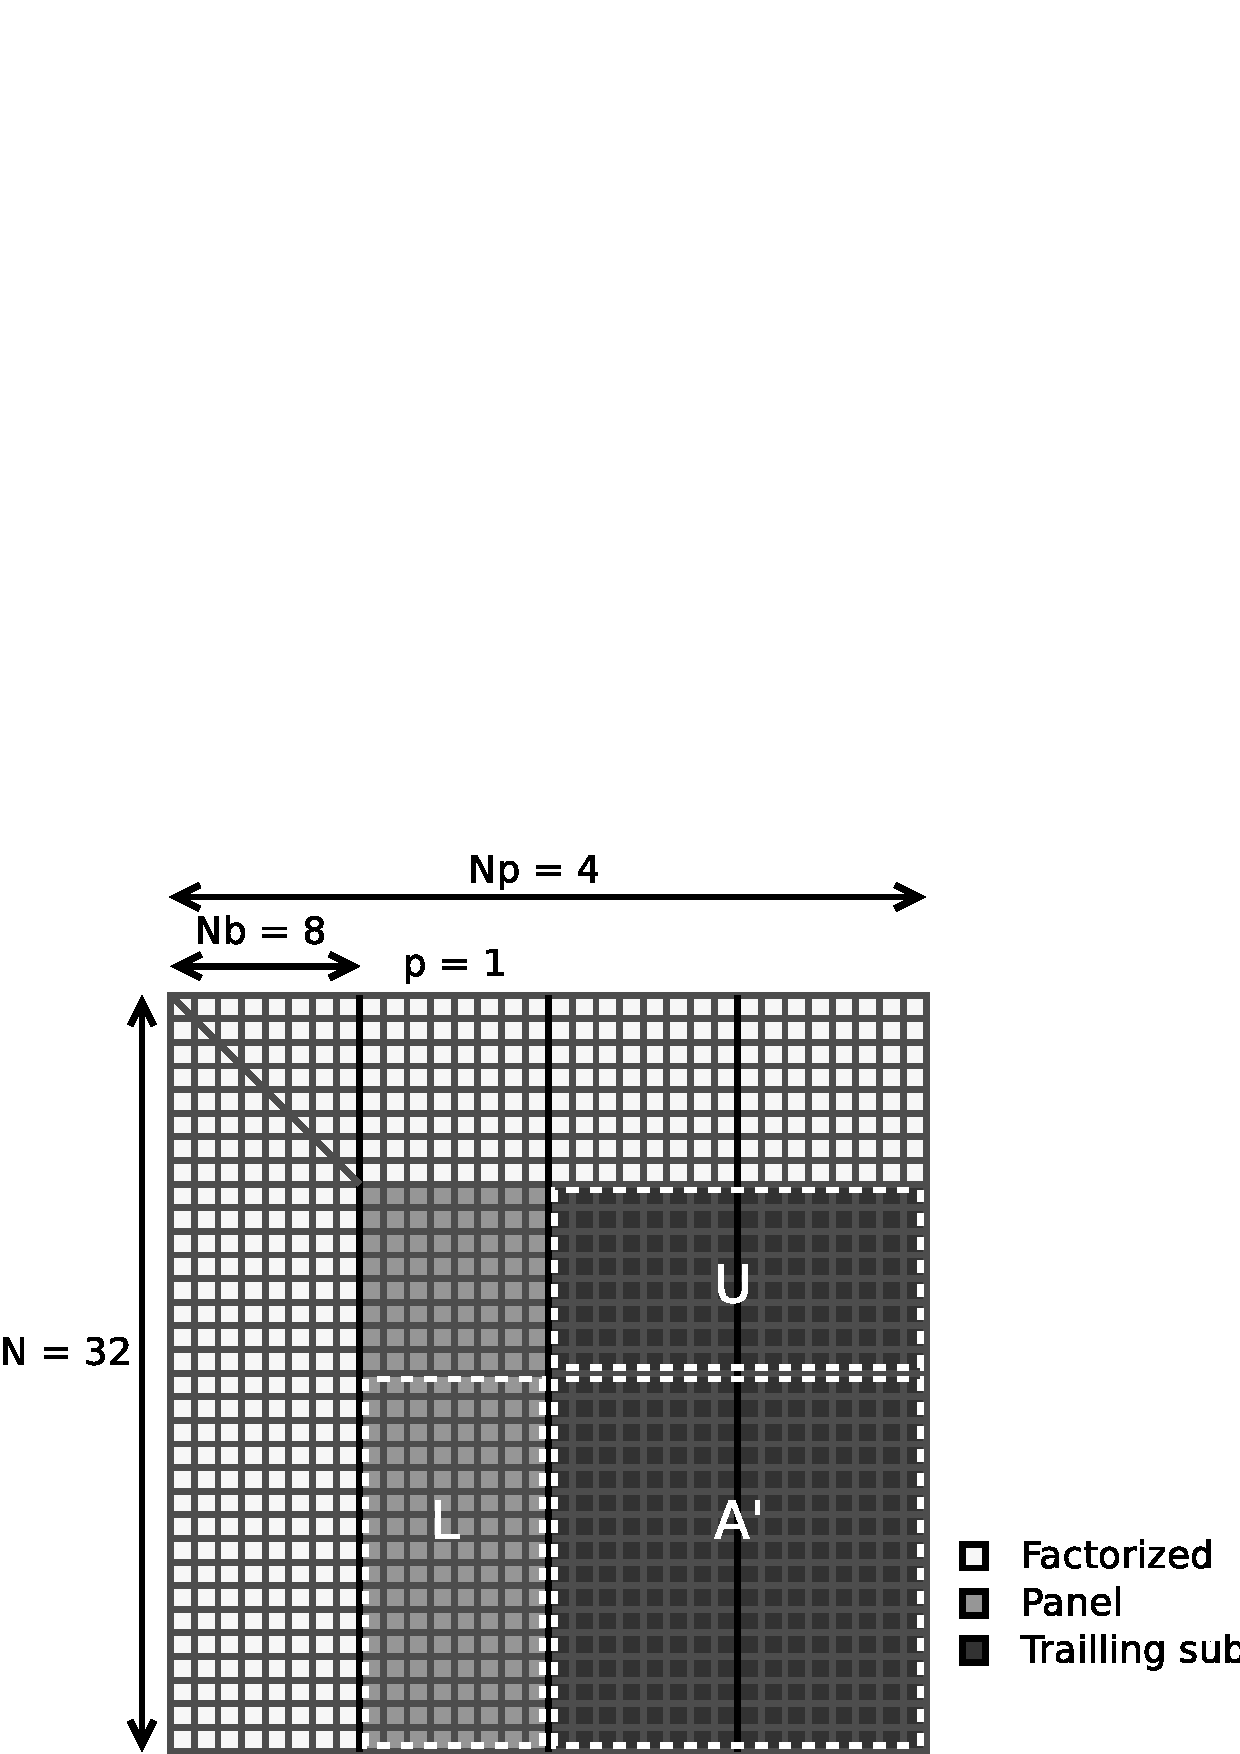
\includegraphics[width=0.9\textwidth]{figures/panel_matrix_bw.pdf}
\caption{LU decomposition at step $p$ on panel-blocked matrix \label{fig:matrix}}
\end{figure}

 
At each step $p$, the panel factorization is performed on the $p^{th}$ panel. Such a panel factorization consists in a loop of $n_b$ iterations. At each iteration $i$ ($p*n_b \leq i < (p+1)*n_b$), a search for the maximum of the $i^{th}$ column is performed, then its row is swapped with the $i^{th}$ row.
Then, a BLAS \textit{scal} routine is applied on the column $i$. It consists to divide all the element of the column $i$ by the selected pivot (Figure \ref{fig:panel} show the different parts of the panel).
After that, the trailing sub-panel is updated with an outer product (\textit{ger}). The panel factorization produces an array of size $n_b$ containing the pivots selected, we note $ipiv$ this array. For each index $x$ of the array $ipiv$, the row $(p*n_b + x)$ will be swapped with the row $(ipiv[x])$.
Mathematically, the panel factorization can be expressed as follows:\\
\begin{tabbing}
For \= $k$ from $1$ to $nb$\\
\> Search for a pivot, do pivoting and store index\\
\> For \=$i$ from $k+1$ to $n$    /*scal operation*/\\
\>\> $a_{i,k} = a_{i,k}/a_{k,k}$\\
\> For \=$i$ from $k+1$ to $nb$   /*ger operation*/\\
\>\> For \=$j$ from $k+1$ to $nb$\\
\>\>\> $a_{i,j} = a_{i,j}-a_{i,k}*_{k,j}$\\
\end{tabbing}

\begin{figure}[!ht]
\centering
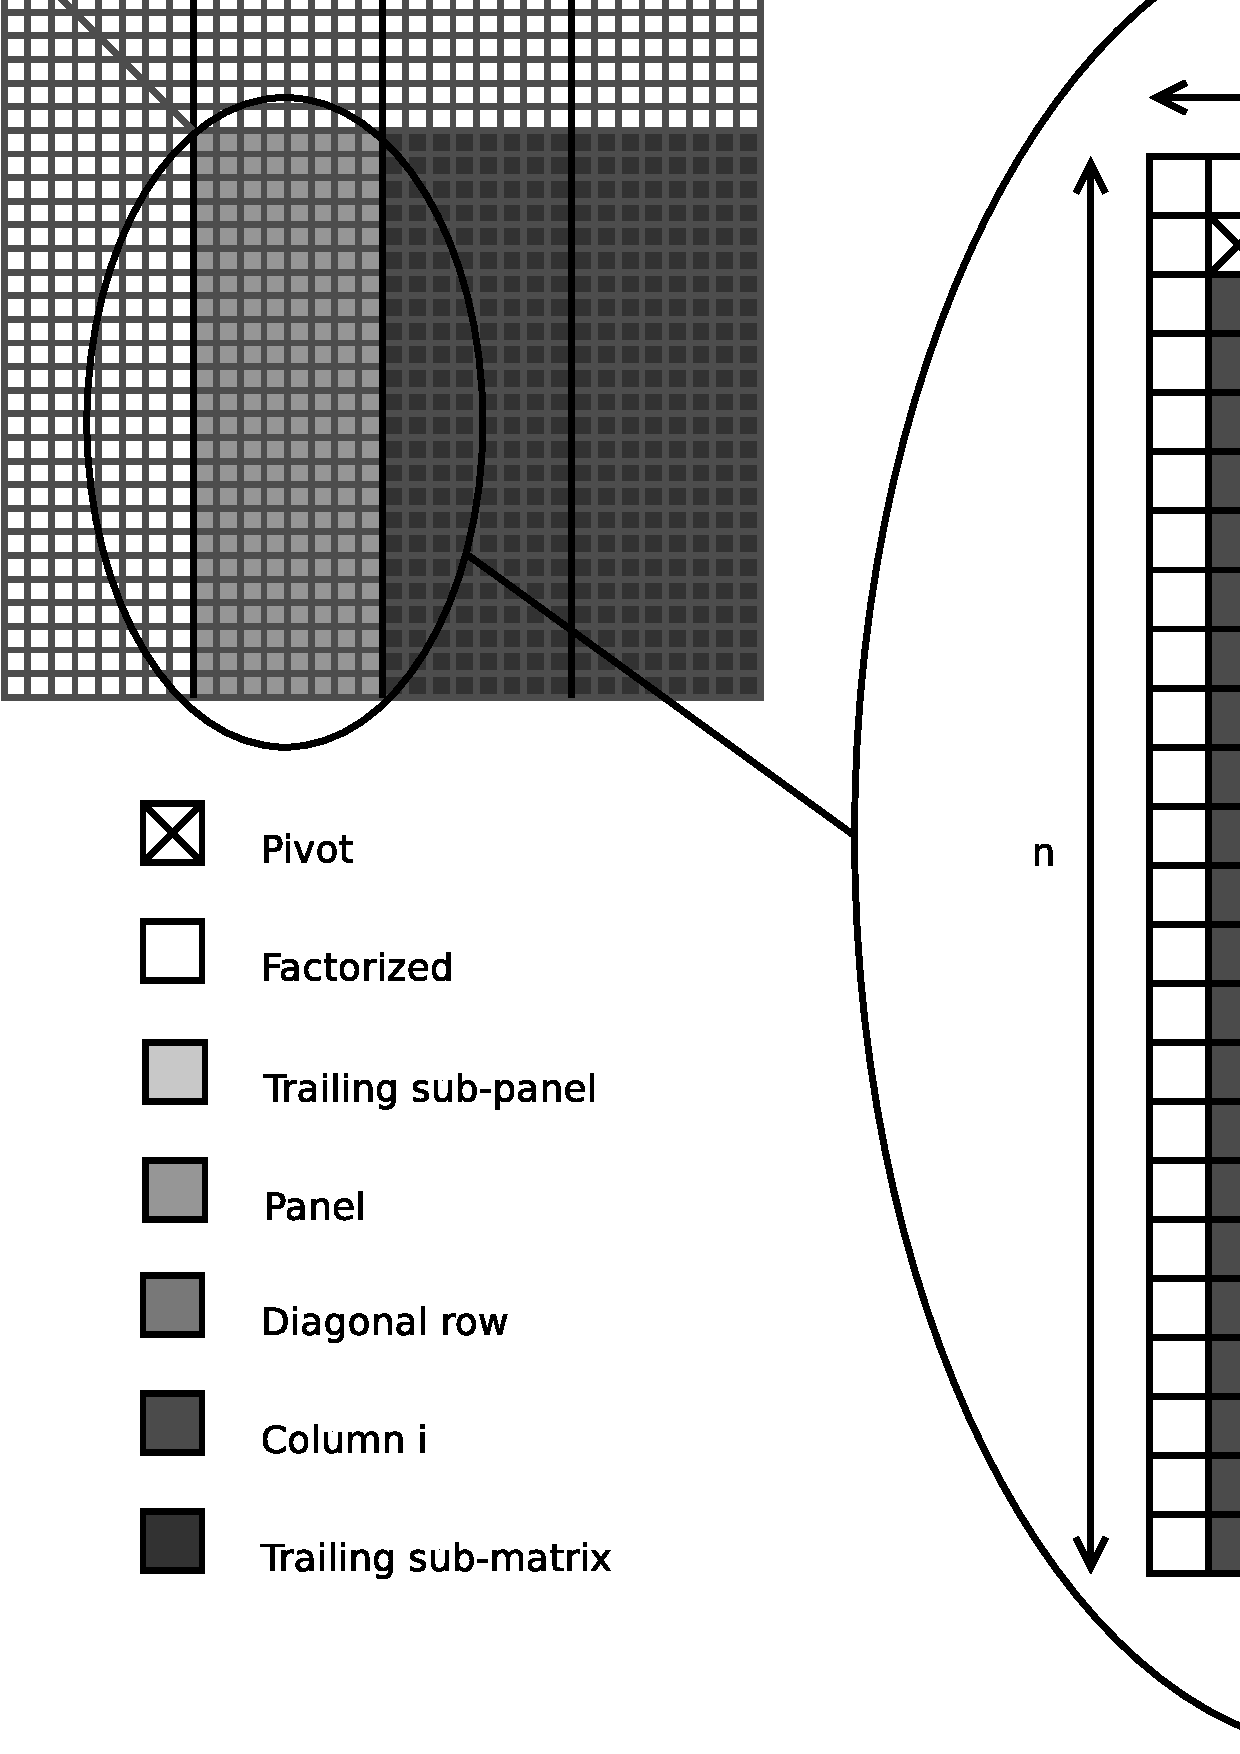
\includegraphics[width=0.8\textwidth]{figures/panel.pdf}
\caption{Second iteration of panel factorization (after swap)\label{fig:panel}}
\end{figure}

Once the $p^{th}$ panel is factorized, the subsequent trailing sub-matrix is updated. This update depends on the result of the corresponding panel factorization. It takes as entry the pivot information and then applies the permutations on the whole trailing sub-matrix. Once the swaps have been performed on the trailing sub-matrix, the $n_b$ block row corresponding to the eliminated rows (block $U'$ in Figure \ref{fig:matrix}) is updated. For that, the following equation must be solved:
\begin{center}
$U'^{(k)} = L*U'^{(k+1)}$
\end{center}
Which is equivalent to:
\begin{center}
$U'^{(k+1)} = L^{-1}*U'^{(k)}$
\end{center}
To solve this equation, we can use the BLAS routine \textit{trsm}. The block $U'$ obtained is then multiplied with the block $L'$ and the resulting matrix is subtracted from the matrix $A'$:
\begin{center}
$A'^{(k+1)} = A'^{(k)} - L'^{(k+1)}*U'^{(k+1)}$
\end{center}
This operation is performed with the BLAS routine for matrix multiplication \textit{gemm} (\emph{ge}neral \emph{m}atrix \emph{m}atrix operation).


\section{Task Flow LU Decomposition over Runtimes \label{task_flow_lu}}
We consider the problem of writing the LU decomposition algorithm as a task flow model in order to be executed over runtime systems (particularly on \dague). In the case of dense linear algebra, the algorithms have been redesigned to cope with this model. They are expressed in terms of tasks operating on fine grain squares sub-matrices, also called tiles \cite{conf/para/ButtariDKLLT06,ChanEtAl07b}. Figure \ref{fig:tiled_matrix} shows a matrix partitioned into tiles. 

\begin{figure}[!ht]
\centering
\includegraphics[width=0.9\textwidth]{figures/tiled_matrix.pdf}
\caption{LU decomposition at step $p$ on tiled matrix \label{fig:tiled_matrix}}
\end{figure}

In case of LU decomposition without pivoting, the tile algorithm is very similar to the blocked panel algorithm of LU decomposition without pivoting. In fact, the panel factorization is split into two tasks: one operating on the diagonal tile (see Figure \ref{fig:tiled_matrix}) and the second performing on the other tiles of the panel. The first one will execute the natural LU decomposition without pivoting algorithm (presented in first part of \ref{algo_lu}), we will call it  \textbf{GETRF} according to \emph{getrf} routine (\emph{ge}neral  \emph{tr}iangular \emph{f}actorization) of Lapack which is a mathematical library build ont the BLAS routines to solve - for example - linear algebra or eigenvalues problems. The second operation has to solve the equation:
\begin{center}
$L'^{(k)} = L'^{(k+1)} * U$\\
$\Updownarrow$\\
$L'^{(k+1)} = L'^{(k)} * U^{-1}$
\end{center}
This can be solved with \emph{trsm} operation. Thus, the task operating this solve will be called \textbf{TRSM\_L}.

As for the blocked panel algorithm, the update is a twofold operation: \emph{trsm} for tiles owning the eliminated rows and \emph{gemm} for the other tiles of the trailing sub-matrix. We will call them respectively \textbf{TRSM\_U} and \textbf{GEMM}.

All these tasks interact by exchanging data. These interactions can be represented by an automate. Figure \ref{fig:automate} shows the automate of tasks interactions of the tile LU algorithm, we can see that the task \textbf{GETRF} takes the diagonal tile as entry to factorize it. If it is the first iteration $k=0$, it takes it directly from the memory, otherwise it takes it from the output $A'$ of the \textbf{GEMM} task of the previous iteration. The resulting tile of the task \textbf{GETRF} - which is two matrix $L$ and $U$ - is respectivly sent to the tasks \textbf{TRSM\_L} and \textbf{TRSM\_U}.

\begin{figure}[!ht]
\centering
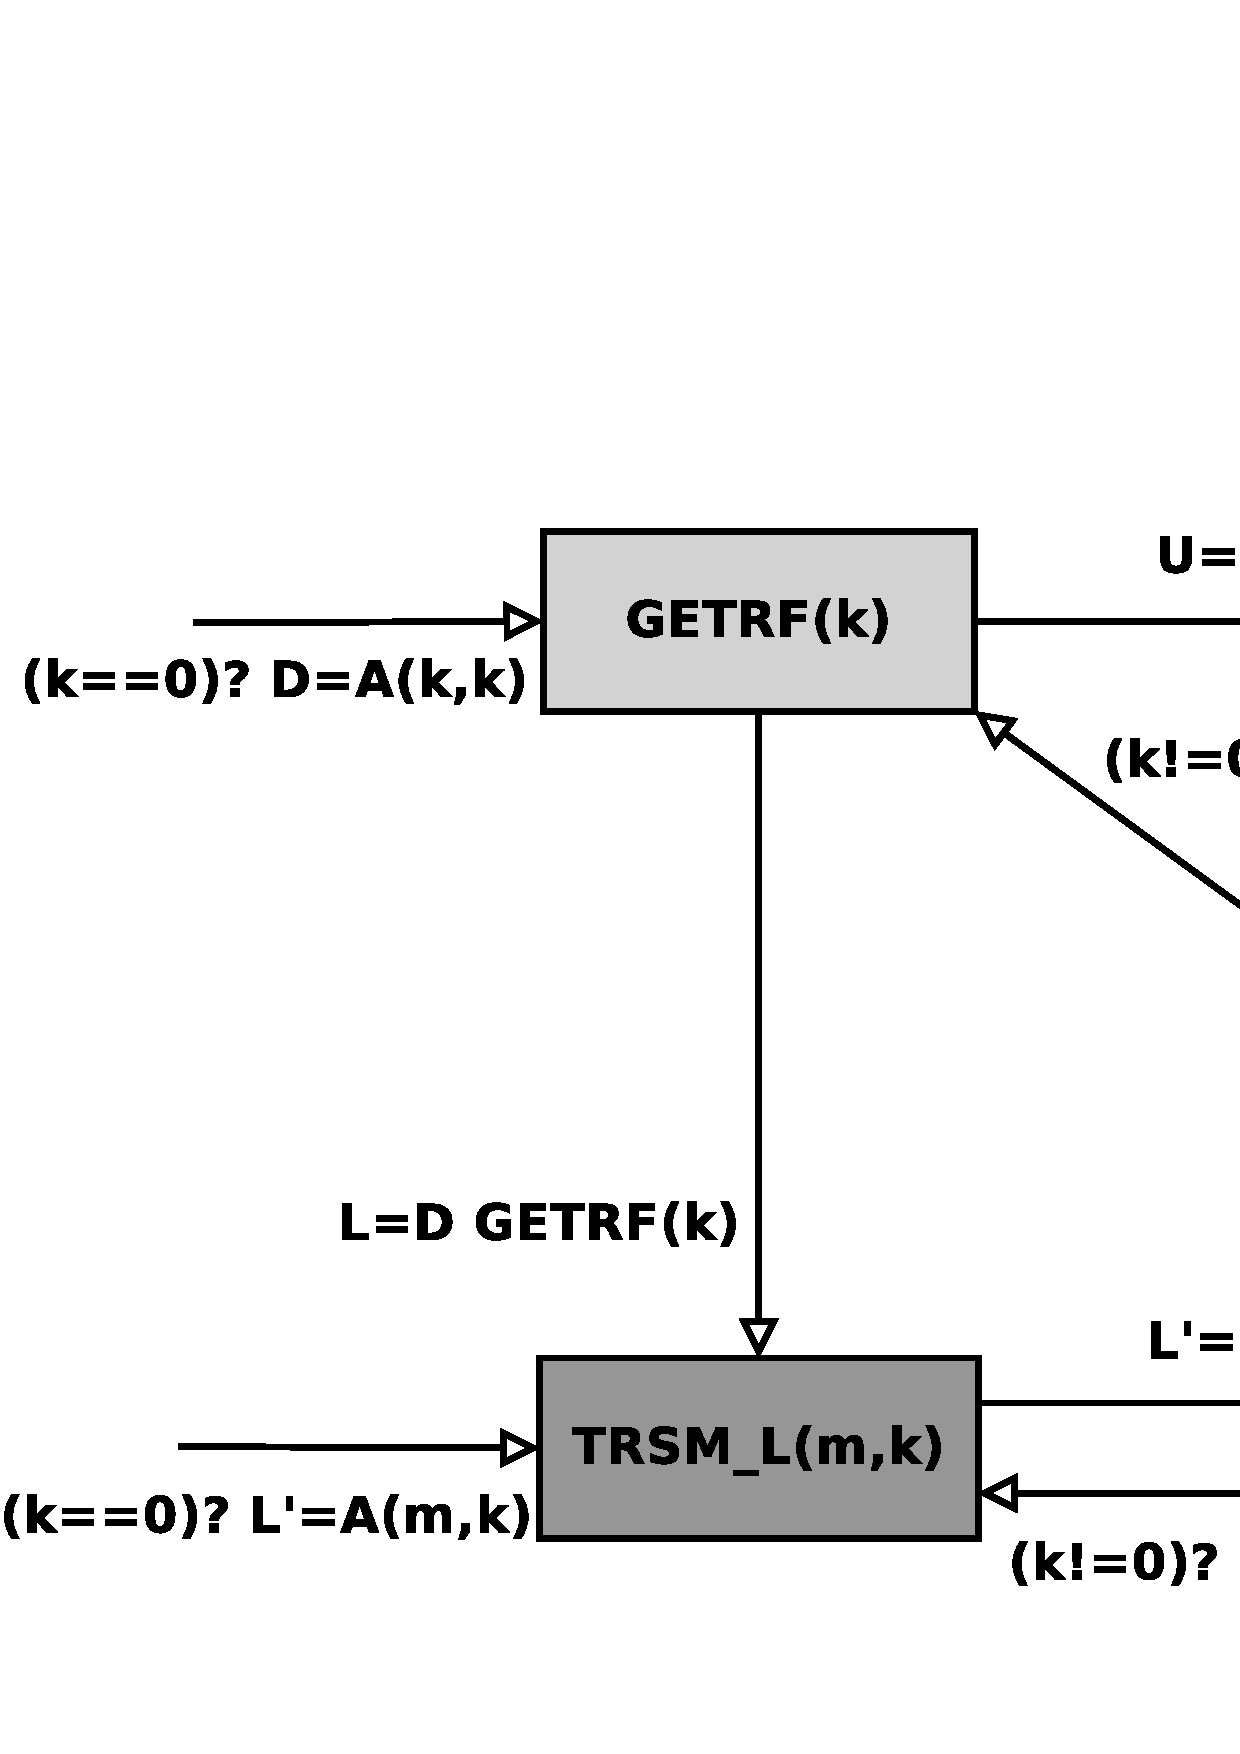
\includegraphics[width=0.9\textwidth]{figures/automate.pdf}
\caption{Automate of tasks interactions of tile LU decomposition algorithm \label{fig:automate}}
\end{figure}

The execution of the automate of interactions provides a DAG of task flow. Figure \ref{fig:dag_dgetrf} shows the DAG obtained after unrolling the automate of Figure \ref{fig:automate} on a matrix of three tiles.

\begin{figure}[!ht]
\centering
\includegraphics[width=0.7\textwidth]{figures/dag_getrf.pdf}
\caption{DAG of the task flow LU decomposition algorithm  on a matrix of 3 tiles \label{fig:dag_dgetrf}}
\end{figure}

As for the blocked panel algorithms, the LU decomposition without pivoting is numerically unstable. In \cite{Buttari09}, the authors proposed a new pivoting strategy called \emph{incremental pivoting} based on \cite{Quintana-Orti:2009:ULF} more suitable to tile algorithms and achieved high performance by limiting the number of synchronizations and enabling more parallelism. The algorithm applies a partial pivoting only on the diagonal tile, then it factorizes sequentially every other tiles of the panel and if a better pivot is found during this decomposition, the upper triangular matrix of the diagonal tile is accordingly updated. The update of the trailing sub-matrix is also done sequentially by using its own routines which are less efficient than \emph{gemm} operations.


However, this algorithm has been proven numerically unstable \cite{journals/siammax/GrigoriDX11}. In order to achieve better stability, we choose to adapt the partial pivoting algorithm to the task flow model.

To illustrate the complexity of implementing the algorithm, we consider the pivot research. This research occurs at each column factorization and lies on the critical path of the decomposition. Partial pivoting requires to select the maximum of the elements below the diagonal in the column. Then, elements lie on $(n-k)/n_b$ different tiles which may be potentially mapped on a huge number of cores in order to ensure state of the art load balancing techniques. The research induces a synchronization at each column which may overwhelm all potential benefits of tile algorithms and deliver too many tasks to be processed by the runtime.

Another issue with the implementation of the partial pivoting algorithm over the task flow model, is the swapping operation of the update. In fact, after receiving the pivots array from the panel factorization, the upper tile has to send the selected rows to other tiles and receive back the substitute ones. If the swap is done rows by rows, the upper tile may exchange a row with another tile of the panel depending on the numerical values of the pivots. The task flow model can thus no longer be statically build in advance but has then to be dynamically composed. Figure \ref{fig:dynamic} represent a simplified task flow of the sending operation with an automaton. Each time the execution of an algorithm will depend on a value of a data, we will call this phenomenon a \emph{data dependency}. The algorithm which contains data dependencies will be called \emph{dynamic algorithm}. These algorithm may be represented by automatons or others conditional mathematical objects. Unfortunately, almost runtimes supports only static representation of task flow (DAG). Thus, the challenge is to represent a dynamic algorithm with a static representation covering the collection of possibilities. A solution is to create a DAG with a path where all concurrent tasks are sequential and move conditions of transitions to the kernel of the tasks. Figure \ref{fig:static} represent the same dynamic algorithm of Figure \ref{fig:dynamic} with a DAG, we can see that all the tasks are represented sequentially and that the conditions of the dependencies are integrated to the kernels. This transformation may increase tremendously the number of tasks and communications required to execute the algorithm. In the next sections we will present how we reduce the size of this static representation to perform the panel factorization and then update the trailing sub-matrix.

\begin{figure}[!ht]
\begin{minipage}[!ht]{.5\textwidth}
\centering
\includegraphics[height=3cm]{figures/dynamic.pdf}
\caption{Dynamic representation of task flow\label{fig:dynamic}}
\end{minipage} \hfill
\begin{minipage}[!ht]{.5\textwidth}
\centering
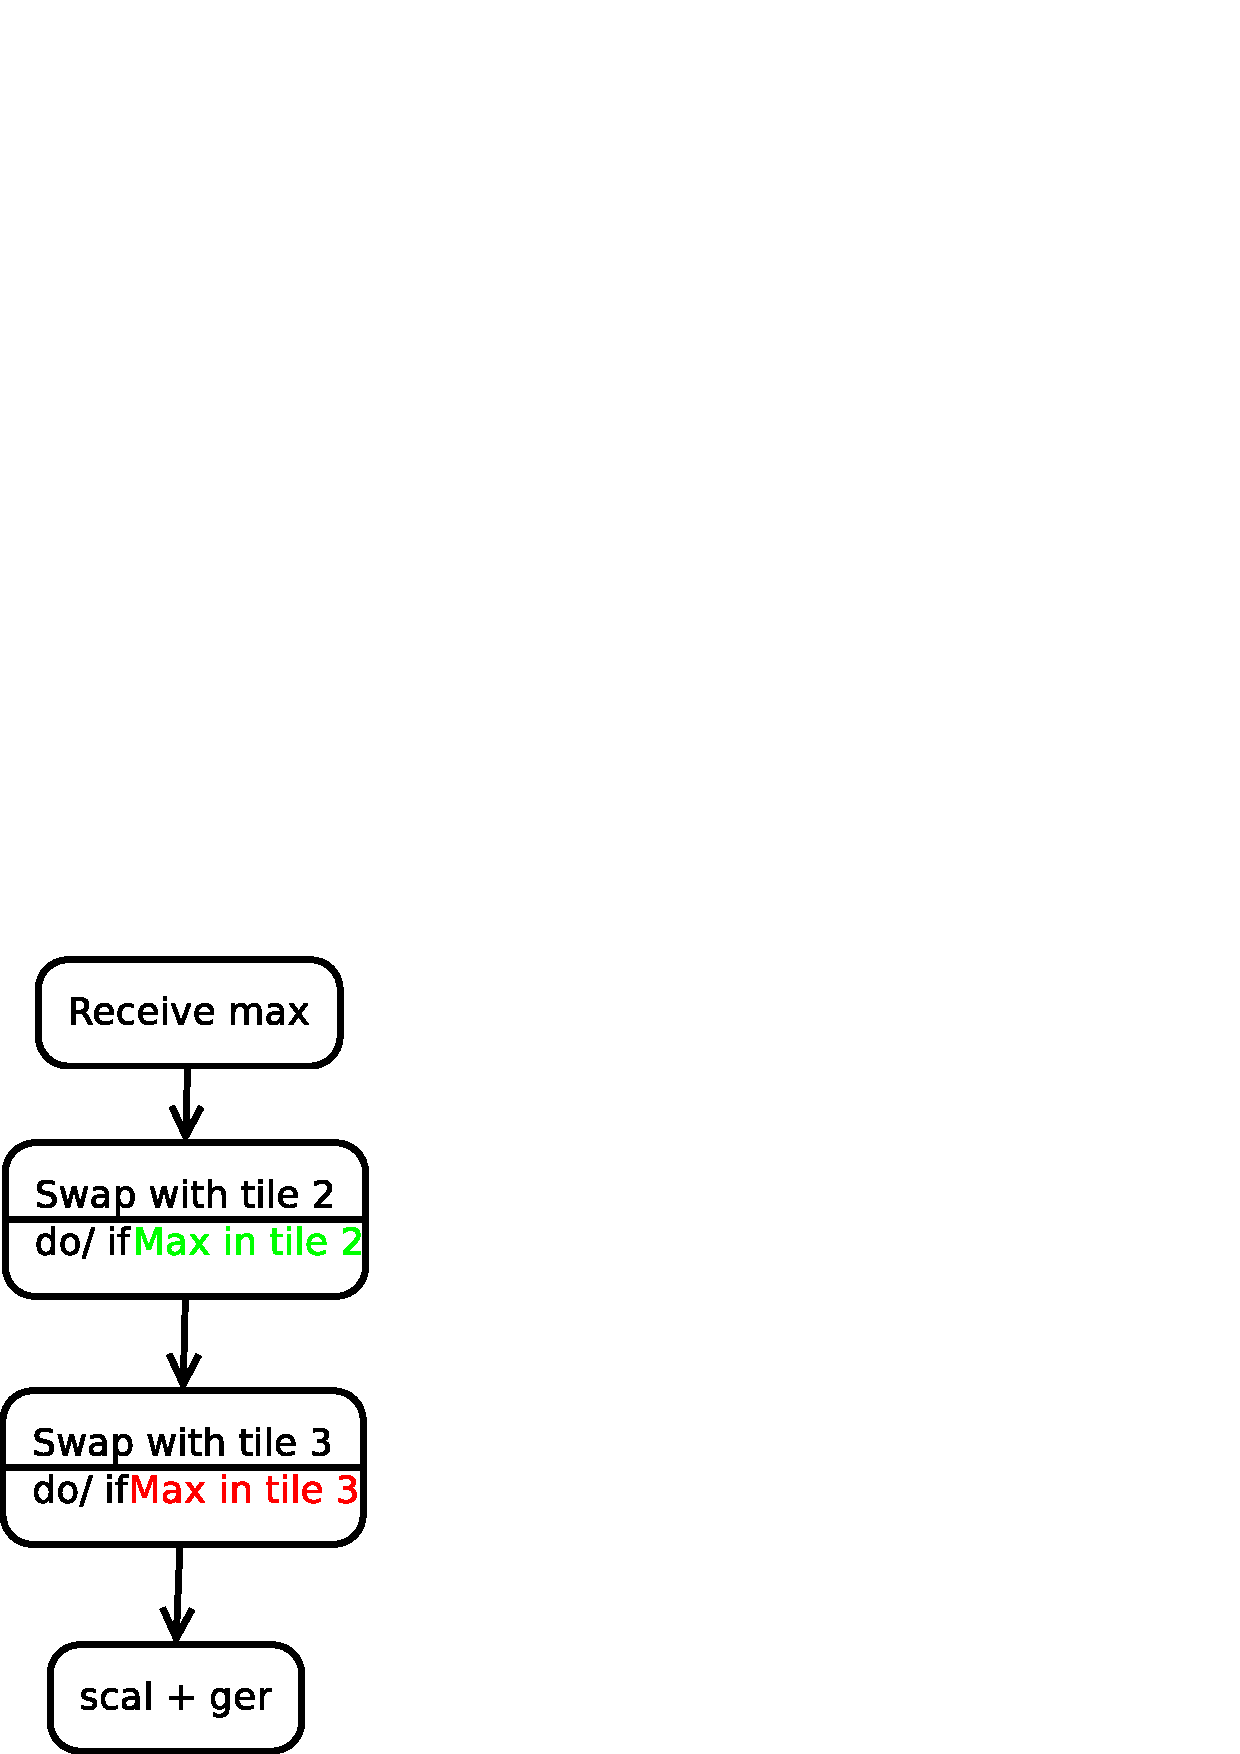
\includegraphics[height=4cm]{figures/static.pdf}
\caption{Static representation of task flow\label{fig:static}}
\end{minipage}
\end{figure}


\chapter{Panel Factorization with Partial Pivoting}\label{panel}
In order to reduce the important number of tasks and communications, optimisations had to be applied at all levels of the algorithm. For that, we present in this section the evolution of the algorithm from the first natural version to the most optimized. As said in the section \ref{lu_algo}, the panel factorisation is a loop of $n_b$ iterations. At each iteration $k$, several operations are executed on the panel.
The first natural version is that the node which contain the diagonal node compare progressively its maximum with others tiles. Each time it find a greater maximum, it save it and use it for next comparisons. After this operation, the diagonal tile broadcast the initial diagonal row and the resulting maximum row to all others tile in order that the concerned tile apply the swap, and every tile apply the \emph{scal} and \emph{ger} operations (Level 1 BLAS) \cite{reference/parallel/X11ab}. Task flow \ref{fig:natural_task_flow} shows one iteration of the panel factorization on a panel of 6 tiles for distributed architecture.

\begin{taskflow}[!ht]
\centering
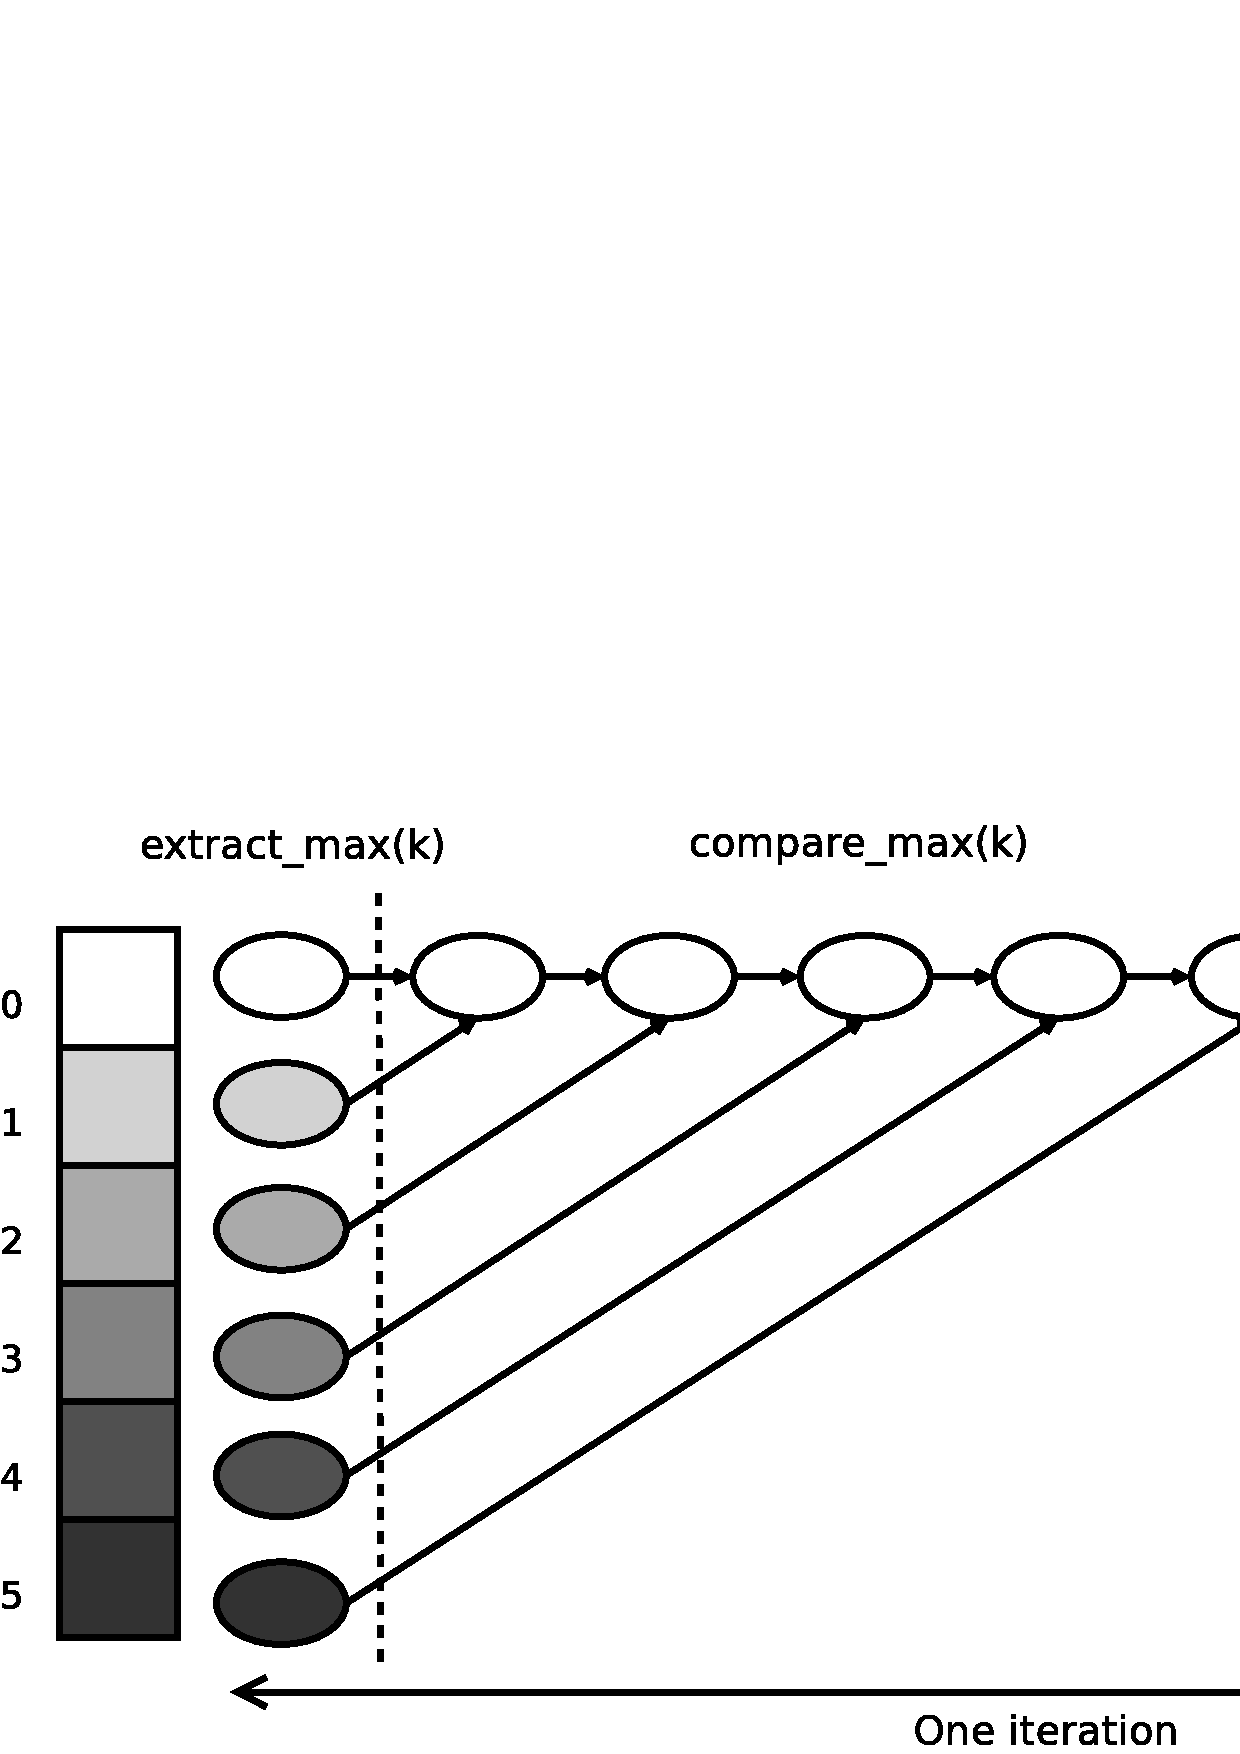
\includegraphics[width=0.8\textwidth]{figures/natural_tf_bw.pdf}
\caption{One iteration of panel factorization on distributed architecture \label{fig:natural_task_flow}}
\end{taskflow}

The first remark is that there is some communications which can be optimized. In fact, instead using an natural sequential comparison, it is possible to use a \emph{reduce} operation. It will allow to perform a faster election of the maximum row. Therefore, because the next operation to the comparison is a broadcast, we can merge the two operations into one single \textit{all\_reduce} operation.

Concerning communications, runtimes handle point-to-point communications and can manage some collective communications as broadcast or group communications. But, to perform more complex communications operations (reduce, gather\dots), we have to express them as a task flow. For the \emph{all\_reduce} operation, the task flow needed is based on the task flow of the Bruck's algorithm \cite{BruckEtAl97}.
In the natural version, we broadcast two rows (the initial diagonal row and the resulting maximum row). Thus, for the \emph{all\_reduce} operation, an array of two rows per node is needed, we will call it a workspace. The first one is filled at beginning by the diagonal tile with the initial diagonal row, and the second row is filled by all tiles with their maximum row. At each step of the \textit{all\_reduce} operation, task copy first row from the received workspace if it is not empty, and reduce the maximum row in the second row of their workspace. Thus, at the end of the \textit{all\_reduce} operation, all workspaces will be filled with the same values.

The second remark is that some tasks can be merged. For that, the \emph{extract\_max} of step $k$ and \emph{scal\_ger} of step $k-1$ tasks can be done in one single task.
The resulting task flow is presented in Task flow \ref{fig:distributed_task_flow}.

\begin{taskflow}[!ht]
\centering
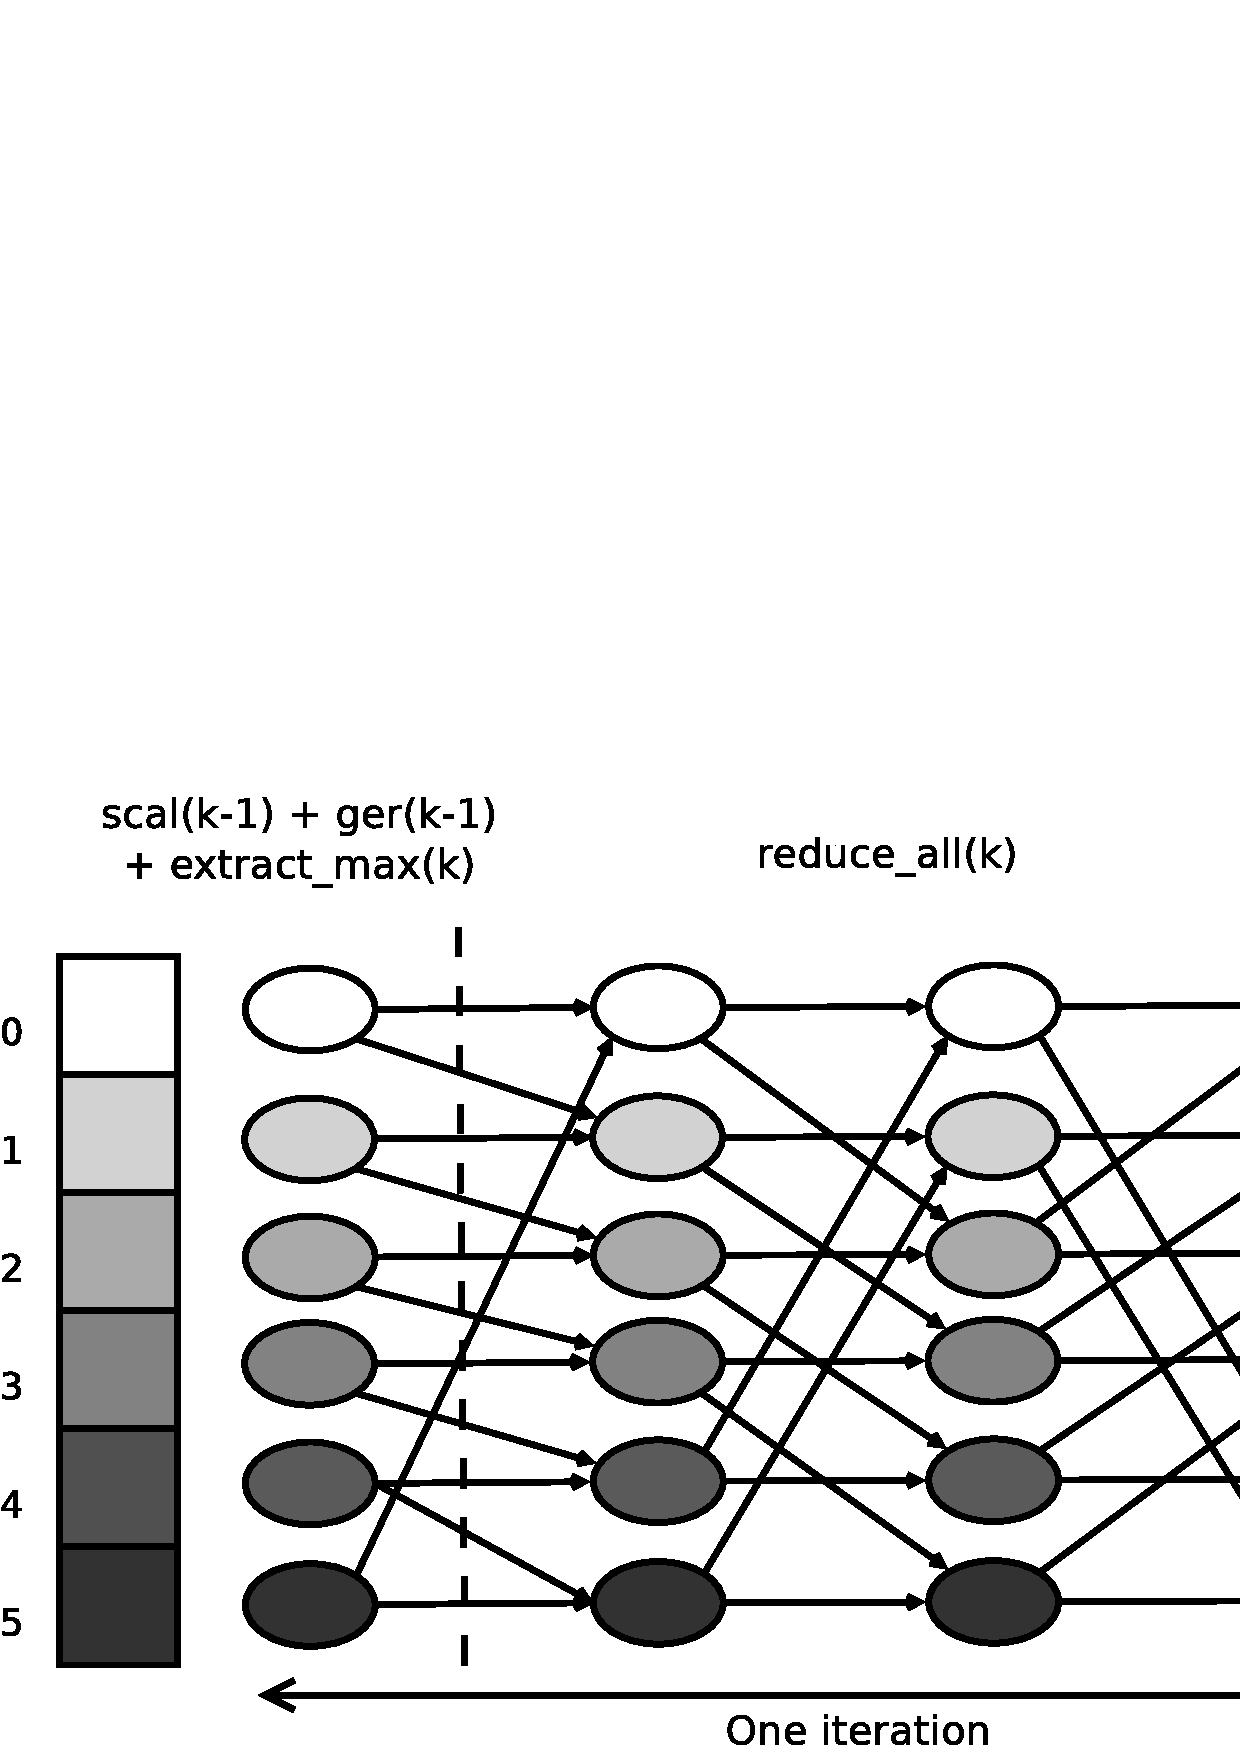
\includegraphics[width=0.6\textwidth]{figures/distributed_tf_bw.pdf}
\caption{One iteration of panel factorization on distributed architecture (combining reduce and broadcast communications)\label{fig:distributed_task_flow}}

\end{taskflow}

Nowadays, most distributed computers contain many cores at each node (see \ref{platform}). To balance well the computations among the processors, a two-dimensional block-cyclic distribution is used to spread the data over the nodes\cite{DGW:SHPCC92}.
If we consider the fact that each node can be multi-core, the task flow \ref{fig:distributed_task_flow} can still be optimized. For that, the idea is to reduce first locally the maximum on the node and then, apply the \emph{all\_reduce} operation between the nodes. The \emph{reduce} operation is performed with a binary tree. Task flow \ref{fig:hybrid_task_flow} shows one iteration of panel factorization for hierarchical architecture. As for task flow \ref{fig:distributed_task_flow}, a similar workspace is used for \emph{all\_reduce} communications with one difference. The workspace contains four rows: two for the diagonal row and two for the maximum row. In fact, at each step of the panel factorization, only one of the two row is used depending on the step parity. This configuration is necessary to protect from the \emph{read after write} effect on the workspace  which is shared between all tiles of the same node.

\begin{taskflow}[!ht]
\centering
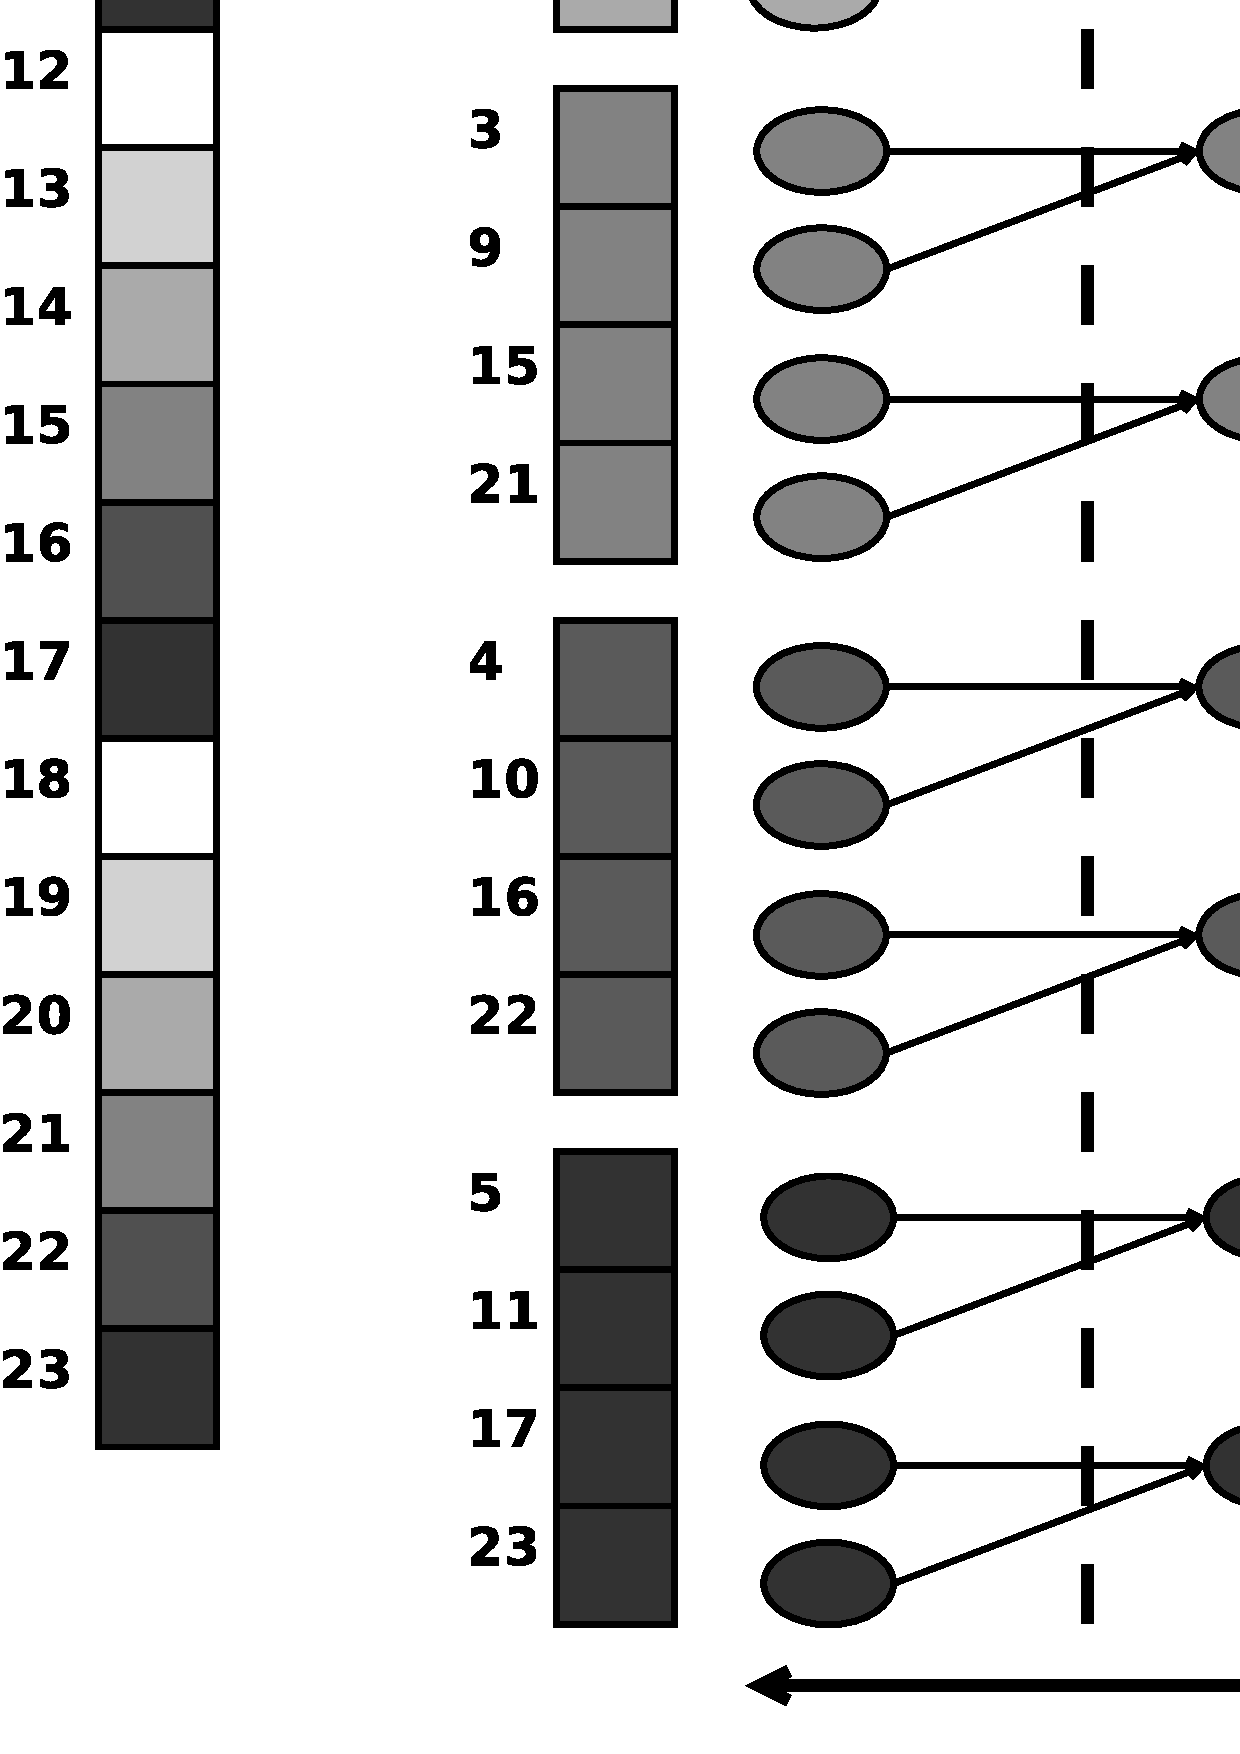
\includegraphics[width=0.7\textwidth]{figures/hybrid_tf_bw.pdf}
\caption{One iteration of panel factorization on hierarchical architecture \label{fig:hybrid_task_flow}}
\end{taskflow}
 
Whether in distributed, shared or hierarchical, the task flow showed in Task flows \ref{fig:distributed_task_flow} and \ref{fig:distributed_task_flow} represent only one iteration of panel factorization. For the last iteration, an additional task is needed to finalize the panel factorization. In fact, this task perform the last \emph{scal} and \emph{ger} operations then release the dependencies to update the trailing sub-matrix.

Beside optimizations in task flow, we apply some optimization on kernel executed by tasks. In case of the task \textit{scal+ger+search\_max}, we use the notion of internal blocking. This optimization is the same applied from linpack to lapack library \cite{Anderson:1990:LPL}. Thanks to the internal blocking, we can use more Level 3 BLAS which increase the performance obtained. In fact, at each step of the panel factorization, instead applying ger on the whole trailing sub-panel, we apply it only on a block. After each $ib$ iterations, $ib$ being the internal blocking parameter, the rest of the trailing sub-panel is updated by a \textit{trsm} and  a \textit{gemm} (Figure \ref{fig:panel_ib}).

\begin{figure}[!ht]
\centering
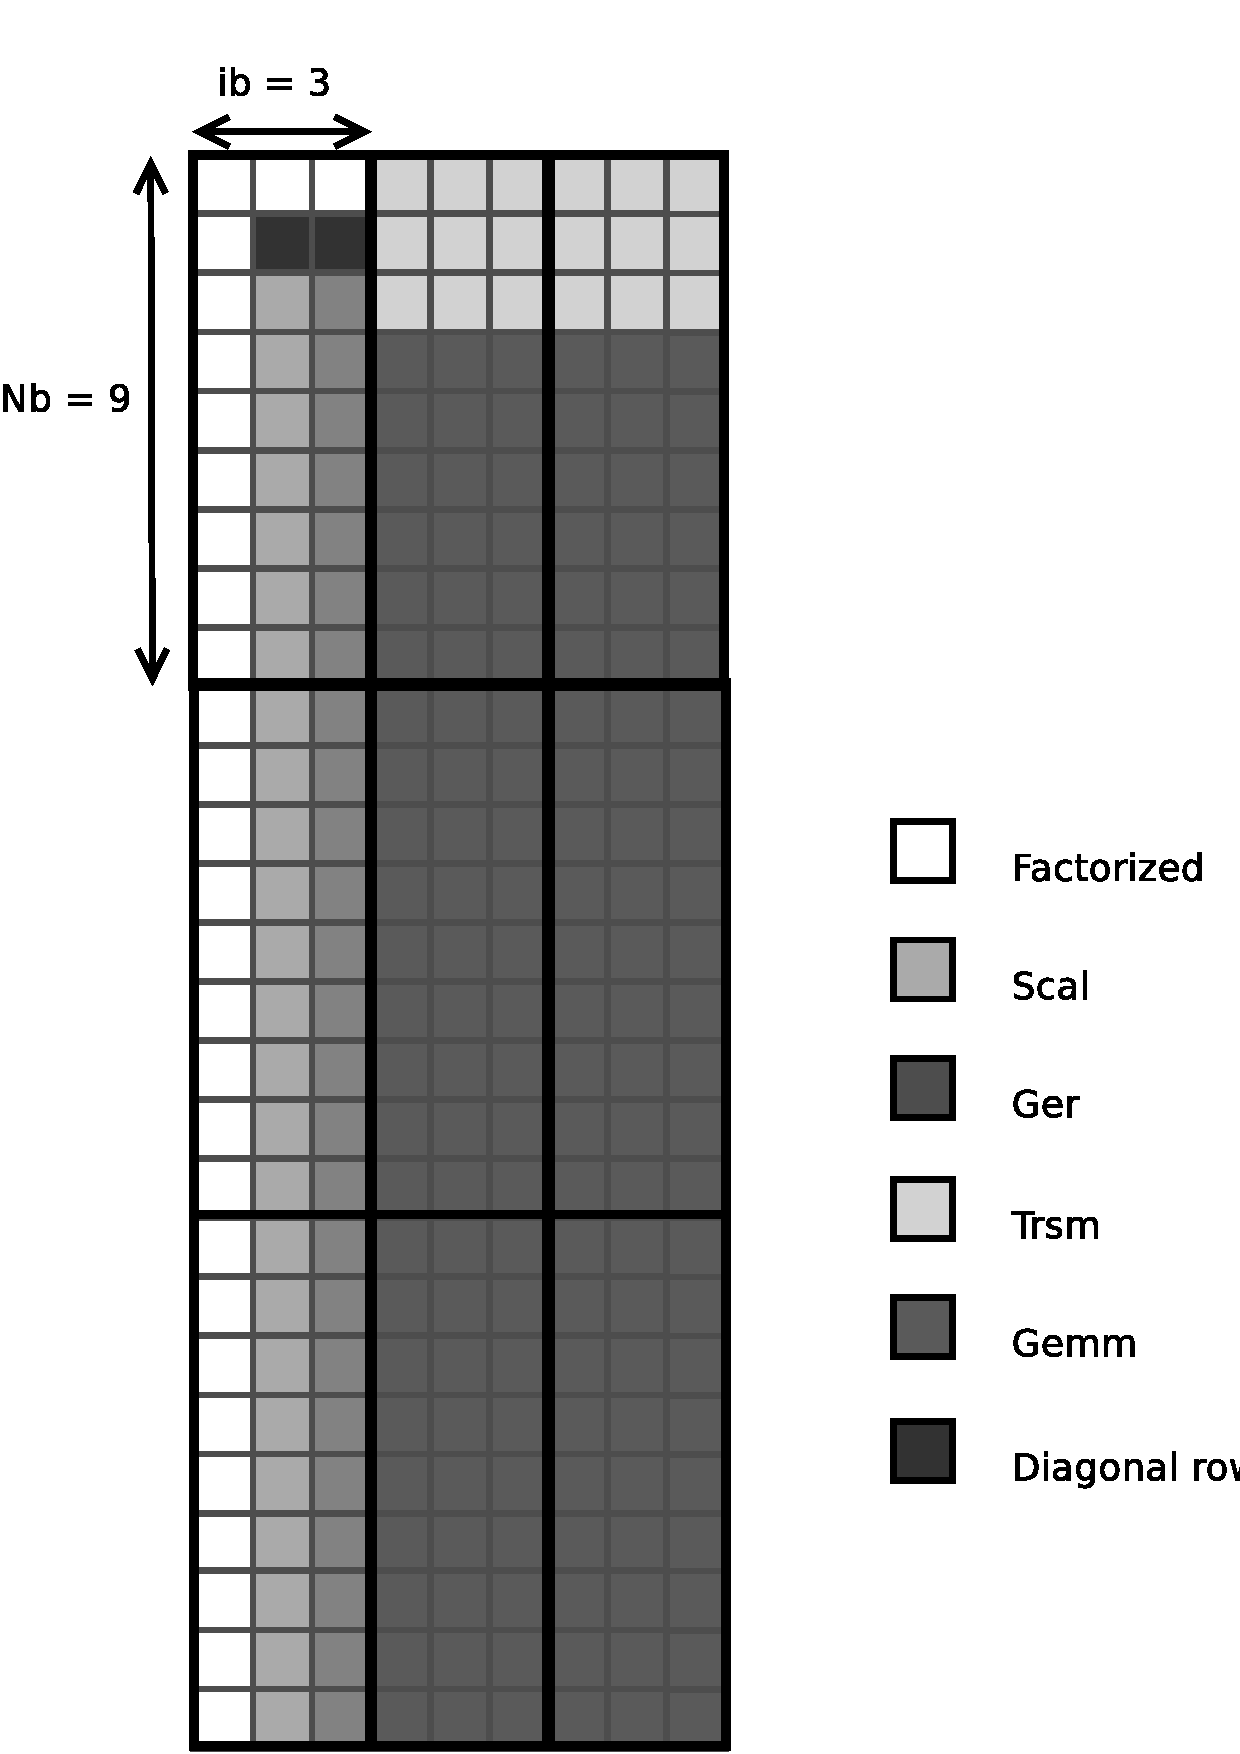
\includegraphics[height=8cm]{figures/panel_ib_bw.pdf}
\caption{Panel factorization with internal blocking\label{fig:panel_ib}}
\end{figure}


\chapter{Update engine for dynamic pivoting}\label{update}
After the panel factorization, the operation performed on the trailing sub-matrix is the update. The update takes the array of pivots produced by the panel factorization, swaps the rows and then apply \textit{trsm} and \textit{gemm} operations.

To perform one swap, the algorithm depend on the value of the pivots, this is what we call data dependency and so the algorithm is a dynamic algorithm (section \ref{task_flow_lu}). The solution to represent a dynamic algorithm with a static DAG of task flow is to make a path with all tasks. In practice, it means that all tiles must participate in swapping even if they are not concerned.
For that, each tile will have a workspace of two arrays: the first to store one row coming from the upper tile and the second to store one row going to the upper tile. Nodes will share between them the workspaces and fill them with the appropriate rows.
The \textit{all\_reduce} seems to be the right operation to use. The cost of a \textit{all\_reduce} operation is $log_2(n_t)$. Thus, the cost of all swaps of one panel is $n_b*log_2(n_t)$. This is very expensive relatively to the cost of SPMD model which is at most $2*n_b$.
Moreover, a the end of each \textit{all\_reduce} operation, only two nodes will really use the rows collected in their workspace (the upper tile and the tile which exchange with it).

A good idea is to perform all swaps at the same time. However, this is not possible with pivots. In fact, because the same row can be several time the maximum row, it is necessary to execute the pivots in the right order (from the first to the last). Figure \ref{fig:pivots} show an example of a row which contains successively two time the maximum row, we can see that the row 1 goes down to the row 13 then comes back to the row 2. Thus, it forces us to perform the first pivots before the second.

\begin{figure}[!ht]
\begin{minipage}[!ht]{.4\textwidth}
\centering
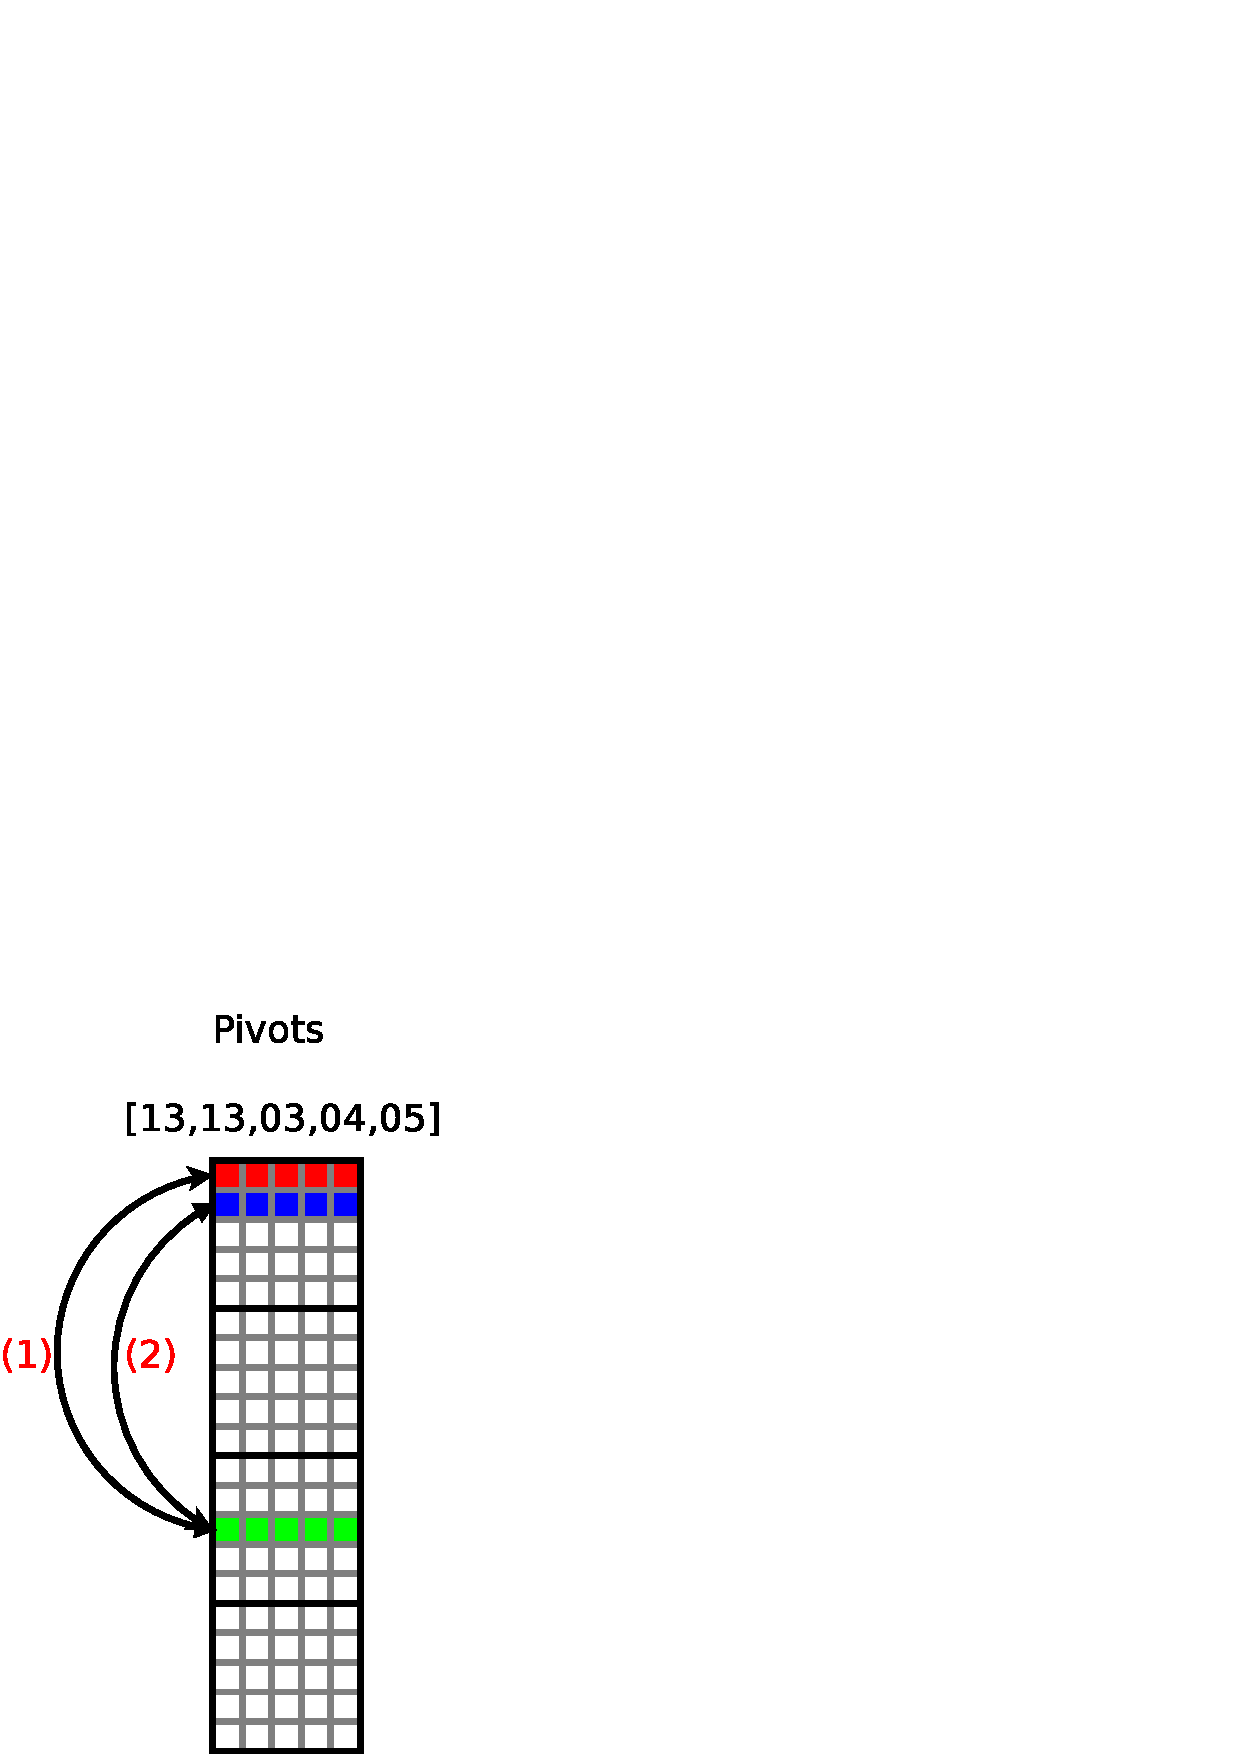
\includegraphics[height=5cm]{figures/pivots.pdf}
\caption{Row movements with pivots\label{fig:pivots}}
\end{minipage} \hfill
\begin{minipage}[!ht]{.4\textwidth}
\centering
\includegraphics[height=5cm]{figures/permutations.pdf}
\caption{Row movements with permutations\label{fig:permutations}}
\end{minipage}
\end{figure}

To reduce high cost of all swaps, the key is to use another structure instead of pivots. For that, the permutations are the right solution. In fact, permutations can be represented by an array of size $n$ (we see after that it can be reduced). For each index $x$ of the array $perm$, the row $perm(x)$ will be moved in place of the row $x$. Thus, with permutations, we know from the beginning the final place of each row. 
Figure \ref{fig:permutations} shows the use of permutations instead of pivots which is showed in Figure \ref{fig:pivots}, we can see that the row 1 goes directly to the row 2 and does	 not move again.
Thanks to this structure, all the rows can be swapped in one single step and the cost will be just $log_2(n_t)$. 
We remark that at most $n_b$ rows go into and from the diagonal tile. Thus, the array of permutations may be limited to a size of $2*n_b$ elements, the fist $nb$ elements will be used to store permutations and the second $nb$ elements will be used to store the inverse of permutations. Therefore, instead of using a workspace of two arrays, it is necessary to use two buffer - with size of tile - for communications: the first is a copy of the upper tile, it is shared from one node to the others. Each node will extracts from the copy rows that it needs. We will call this operation \emph{swap from}. The second buffer is used to gather rows required by the upper tile. Each node create its own buffer, fill it with rows intended to be stored in the upper tile and then participate with it in a \textit{gather} operation. This operation will be called \emph{swap into}. This solution allow us to perform the \emph{swap from} and the \emph{swap into} in parallel.

Task flow \ref{fig:distributed_update_task_flow} represents the swapping operation of update operation for distributed architecture. The bold arrows show some dependencies which add synchronizations to avoid \emph{read after write} effects. For example, the copy of the upper tile must be applied before its update.

\begin{taskflow}[!ht]
\centering
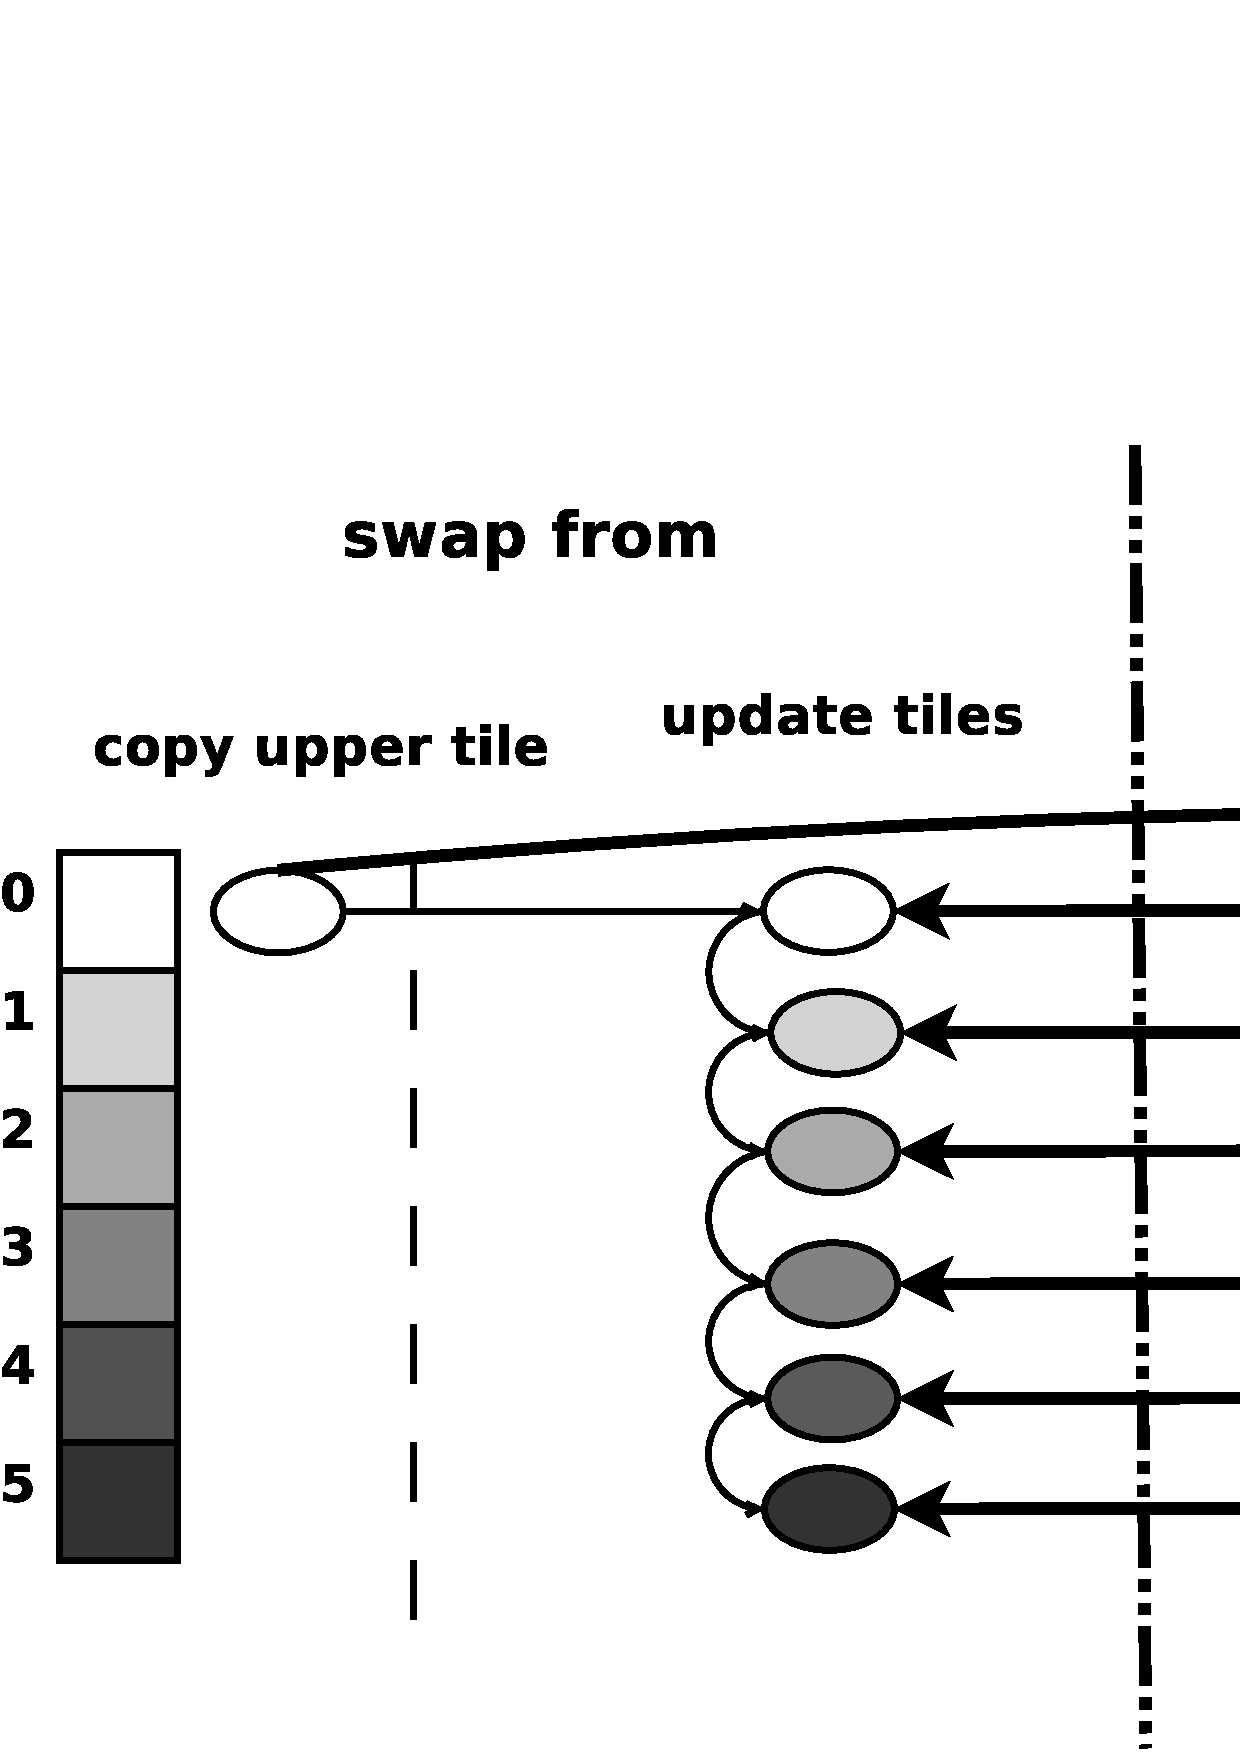
\includegraphics[width=0.8\textwidth]{figures/distributed_update_tf_bw.pdf}
\caption{Swapping operation of update on distributed architecture \label{fig:distributed_update_task_flow}}
\end{taskflow}

As for the panel factorization, we consider that nodes can be multi-core. In order to reduce global communication, each node share its buffers over its local tiles before to send them to others nodes. Task flow \ref{fig:update_task_flow} shows the update operation for hierarchical architecture.

\begin{taskflow}[!ht]
\centering
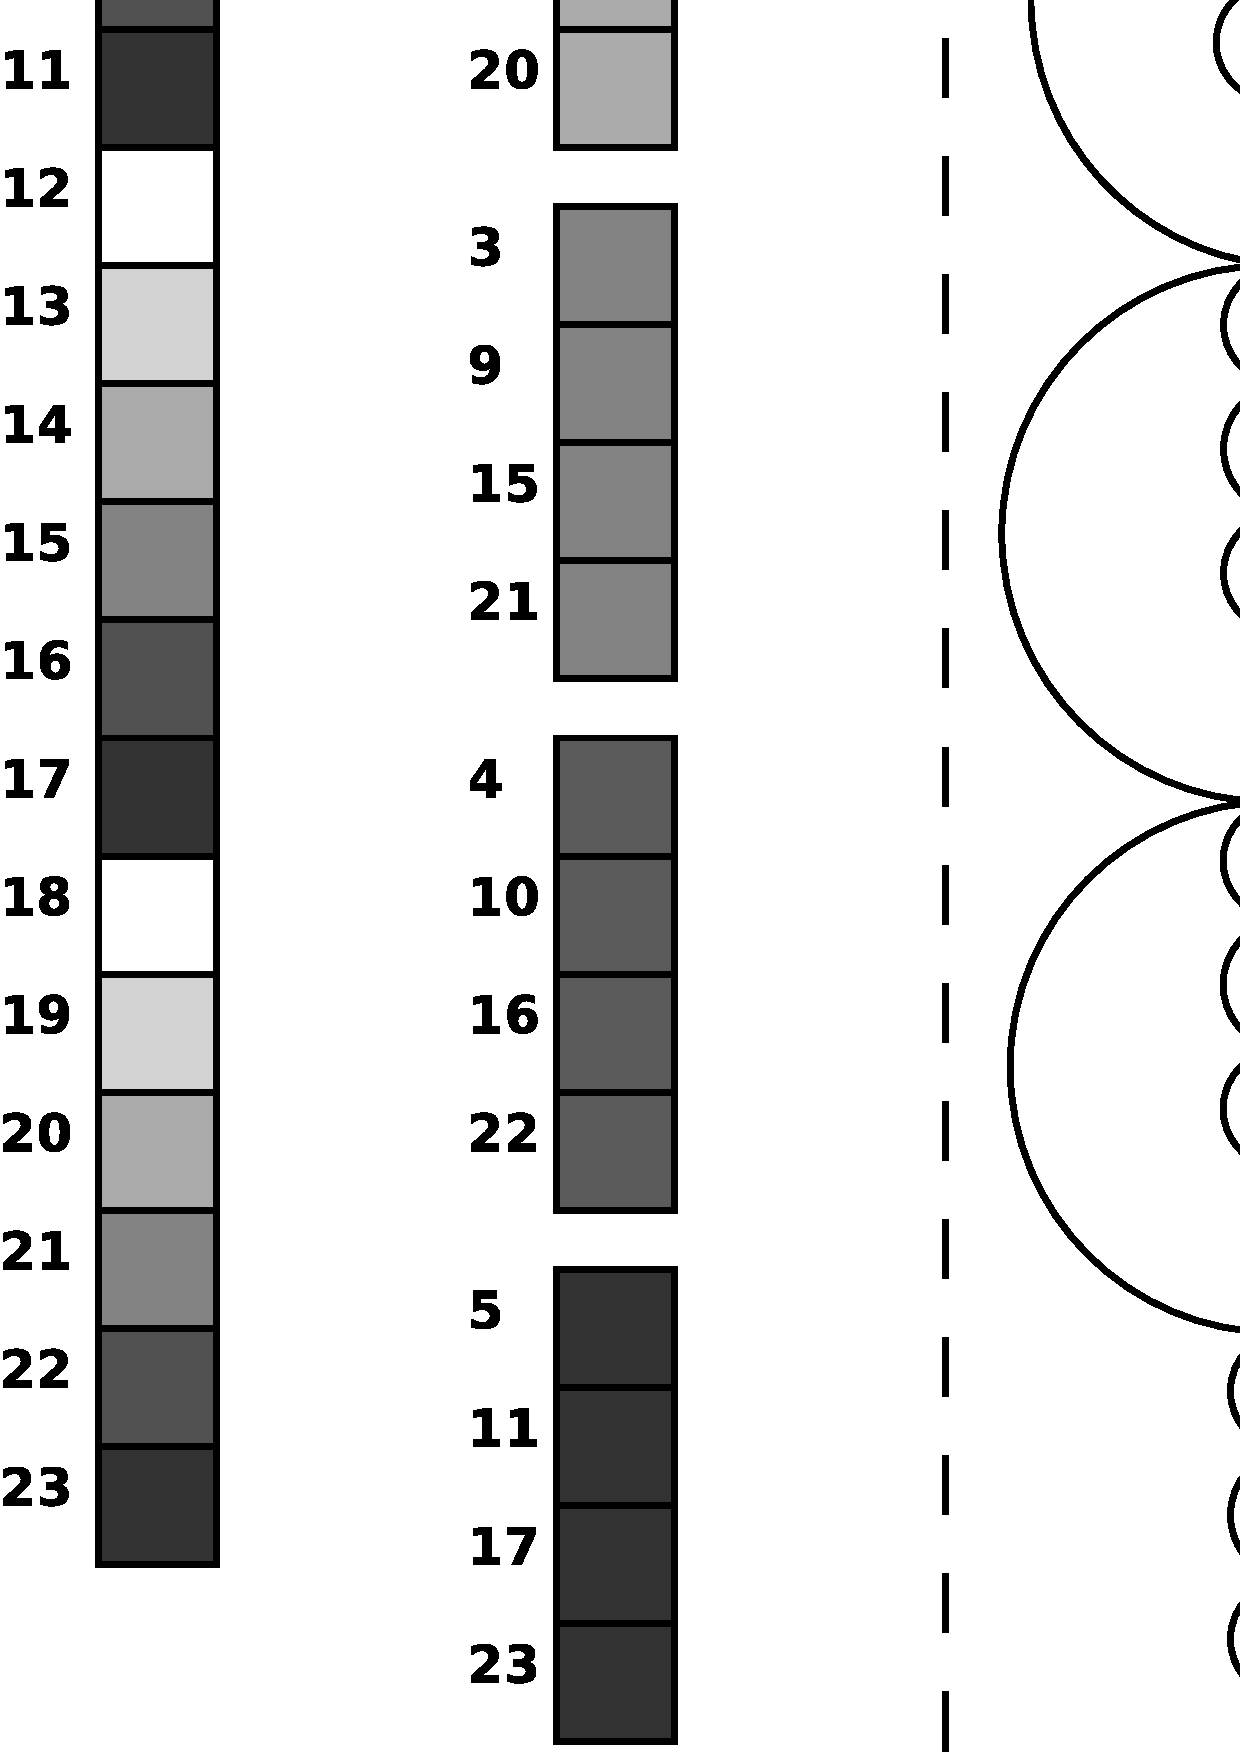
\includegraphics[width=0.8\textwidth]{figures/update_tf_bw.pdf}
\caption{Swapping operation of update on hierarchical architecture \label{fig:update_task_flow}}
\end{taskflow}

Moreover, this update algorithm implemented is a generic solution that it can execute update operation after any panel factorization which provide an array of pivots (incremental pivoting, CALU \dots).


\chapter{Experimental}\label{experimental}
In order to have an upper bound for the LU decomposition with partial pivoting, we also implemented an LU decomposition with static pivoting. It is similar to a partial pivoting but without swapping operation. It may be considered as a Cholesky's algorithm applied to the two sides of the matrix.

\dague and StarPU include already an implementation of LU decomposition with incremental pivoting. Thus, we compare them with the performances obtained of partial pivoting.

To complete the experiences, we also compare results with Scalapack performances.

\section{Exploiting hierarchical platform with PTG}
For this experience, we used \dague as PTG runner. The architecture used is and hierarchical platform. It consists of 128 cores distributed over 16 nodes and interconnected with an Infini Band. Thus, we implemented Task flow \ref{fig:hybrid_task_flow} for panel factorization and Task flow \ref{fig:update_task_flow} for swapping operations in update. The software used is Linux as operating system, \dague as runtime system and Intel Mkl library for Blas routines.

\begin{figure}
\centering
\includegraphics[width=0.8\textwidth]{figures/partial_pivoting_problem.pdf}
\caption{Impact of the update engine on the performances\label{fig:pp}} 
\end{figure}


\section{Exploiting heterogeneous platform with sequential task flow}
%The distributed tests was applied on a machine of 16 nodes of 8 cores each, using an Infini Band network and the Intel MKL library.
%The first experiment applied was to take the static pivoting and plug on it the update engine implemented. Because all communications are done in every case, this test give the cost of the execution of the update engine. The result is showen in the figure \ref{fig:update}. The first remark is that the static pivoting is quickly approaching the gemm peak computer. This can be explained by the fact that all the getrf and trsm operations are recovered by gemm. The second curve is just a little below the first one. Thus, the update engine has a very small impact on the performances despite of its entire execution.  This is a very good result because first the update engine is generic and second its cost is very low.
%\begin{figure}
%\centering
%\includegraphics[width=0.8\textwidth]{figures/dgetrf_update_problem.pdf}
%\caption{Impact of the update engine on the performances\label{fig:update}} 
%\end{figure}
%The second experiment applied was the testing of the LU decomposition with partial pivoting implemented. It was compared to the incremental pivoting and the Scalapack implementation. At the moment, the partial pivoting implemented was runned with only 7 cores by node for computation. The eighth core was completly dedicated to the communication. This was necesary to manage the high number of small communications on the panel. In the figure \ref{fig:pp}, it is showed two gemm peak, one using 8 core and the other only 7.
%\begin{figure}
%\centering
%\includegraphics[width=0.8\textwidth]{figures/partial_pivoting_problem.pdf}
%\caption{Impact of the update engine on the performances\label{fig:pp}} 
%\end{figure}


\chapter*{Conclusion}\label{conclusion}
LU decomposition with partial pivoting is a dynamic algorithm with its data dependencies in the swapping operation for the update. Despite this difficulty, we managed to implement a task flow LU decomposition with PTG and obtained hopeful performances.

We try now to optimize the \dague runtime system to better manage the small communications messages, in order to take full advantage of all cores of nodes. We will be able to have one of the most efficient LU decomposition implementation. Beside its use for resolving system of linear equations, it will be possible to create a new benchmark to analyse computers performances.

In parallel, we implemented another task flow LU decomposition on StarPU. In fact, StarPU runtime allow to implement dynamic algorithm  thanks to its task insertion system. We will be able to compare results to PTG in general and \dague particularly.

\bibliographystyle{splncs}
\bibliography{report}

\end{document}

